\documentclass[letterpaper,journal]{IEEEtran}
\usepackage{amsmath,amsfonts}
\usepackage{algorithmic}
\usepackage{array}
\usepackage[caption=false,font=normalsize,labelfont=sf,textfont=sf]{subfig}
\usepackage{textcomp}
\usepackage{stfloats}
\usepackage{url}
\usepackage{verbatim}
\usepackage{graphicx}
\hyphenation{op-tical net-works semi-conduc-tor IEEE-Xplore}
\def\BibTeX{{\rm B\kern-.05em{\sc i\kern-.025em b}\kern-.08em
    T\kern-.1667em\lower.7ex\hbox{E}\kern-.125emX}}
\usepackage{balance}
\usepackage{newtxtext}
\usepackage{newtxmath}
\usepackage{float}
\usepackage{tabularx}
\usepackage{makecell}
\usepackage{lipsum}
\usepackage{xcolor}
\usepackage{placeins}
\usepackage{datetime}
\usepackage{enumitem}
\usepackage{svg}
\usepackage[switch]{lineno}
\newdateformat{monthyeardate}{\monthname[\THEMONTH] \THEYEAR}

\linenumbers

% correct bad hyphenation here
\hyphenation{op-tical net-works semi-conduc-tor}


\begin{document}
%
% paper title
\title{E-PSS: the Extended Polarimetric Slope Sensing technique for measuring ocean surface waves}

\author{Nathan~J.~M.~Laxague,~\IEEEmembership{Member,~IEEE,}
        Z.~G\"oksu~Duvarc\i,\\
        Lindsay~Hogan, Junzhe~Liu,
        Christopher~Bouillon, and Christopher~J.~Zappa% <-this % stops a space
\thanks{N. J. M. Laxague is with the Department
of Mechanical Engineering and Center for Ocean Engineering, University of New Hampshire, Durham, NH, USA e-mail: Nathan.Laxague@unh.edu.}% <-this % stops a space
\thanks{Z. G. Duvarc\i~ is with the Center for Ocean Engineering, University of New Hampshire; L. Hogan and C. J. Zappa are with Lamont-Doherty Earth Observatory of Columbia University; C. Bouillon is with Institut des Sciences de la Mer, Université du Québec à Rimouski, Rimouski, QC, Canada.}% <-this % stops a space
\thanks{Manuscript received XXX; revised YYY.}}

% The paper headers
\markboth{IEEE Journal of Selected Topics in Applied Earth Observations and Remote Sensing,~Vol.~XX, No.~YY, \monthyeardate\today}%
{Laxague \MakeLowercase{\textit{et al.}}: Subpixel Variability and Polarimetric Slope Sensing}

% make the title area
\maketitle

% As a general rule, do not put math, special symbols or citations
% in the abstract or keywords.
\begin{abstract}
Polarimetric slope sensing (PSS) is a powerful tool for remote measurement of the spatiotemporal characteristics of short surface waves. However, two key shortcomings have negatively impacted the widespread adoption of the technique: (1) the quality of the measurement may be sensitive to variability in environmental illumination conditions and (2) waves longer than the imager field of view are not reliably measured. We present an extension of PSS-- namely, the Extended Polarimetric Slope Sensing (E-PSS) technique, which is robust to variation in ambient illumination conditions and provides simultaneous access to the directional spectrum for both long and short waves from a single surface-looking, narrow FOV camera. 
\end{abstract}

% Note that keywords are not normally used for peerreview papers.
\begin{IEEEkeywords}
Polarimetry, gravity-capillary waves, wave slope sensing, polarimetric slope sensing, division of focal plane
\end{IEEEkeywords}

% For peerreview papers, this IEEEtran command inserts a page break and
% creates the second title. It will be ignored for other modes.
\IEEEpeerreviewmaketitle

\section{Background}
\label{sec:intro}
\IEEEPARstart{T}{here} is a long-standing and pressing need to measure the spatiotemporal characteristics of short-scale (wavelengths smaller than 10 m) surface waves. This is primarily driven by the intimate connection between these intermediate to small-scale waves and the local wind forcing: surface waves with wavelengths between 1 cm to 10 m support a significant fraction of the wave form drag, making them an essential mediator of air-sea momentum flux. It is fortuitous that radar-based remote sensing techniques operate with electromagnetic wavelengths in this very range; specifically, from HF radar down to $k_u$ band microwave scatterometry. This enables indirect measurement of wave height, surface roughness, and wind forcing through interpretation of backscattered power.

However, the most commonly available techniques for measuring the surface wave field are unable to adequately characterize the energy or directionality of the surface wave field at scales shorter than 10 meters. Surface buoys are by far the most ubiquitous of \emph{in situ} wave sensors, but even the small form-factor Spotter buoys do not provide reliable directional information beyond frequencies of 0.8 Hz (roughly corresponding to surface wave scales of 2 to 3 meters). This leaves a great deal of the surface wave spectrum which remains broadly inaccessible to observation. There are several techniques which have been developed to push the resolution of wave measurements to smaller and smaller scales. Perhaps the most widely adopted of these is stereophotogrammetry \cite{Benetazzo2006,bergamasco_wass_2017}. This technique is able to recover the spatiotemporal characteristics of surface waves ranging in scale from 100 meters down to 50 centimeters. While this is quite impressive, it still does leave unresolved short-gravity and gravity capillary waves. Polarimetric slope sensing (PSS) was developed by Zappa and colleagues in 2008 \cite{Zappa2008} following decades of development of the application of classical optical theory towards inferring the shape of a free surface from the polarization state of light reflected off of it. PSS exploits the known (or at least, modeled) relationship between the polarization state of light reflected off an air-water interface and the geometry of the reflecting facet. When repeated spatially (over an imager field of view) and temporally (in short succession, as with video), one is able to recover the spatiotemporal evolution of the wave field down to very fine scales. Nevertheless-- this technique is susceptible to variation in illumination conditions. And as initially presented, PSS could reliably measure the slopes of surface waves with wavelengths ranging from a few millimeters up to one meter (but in practice, rarely larger).

\begin{figure}[!ht]
    \centering
    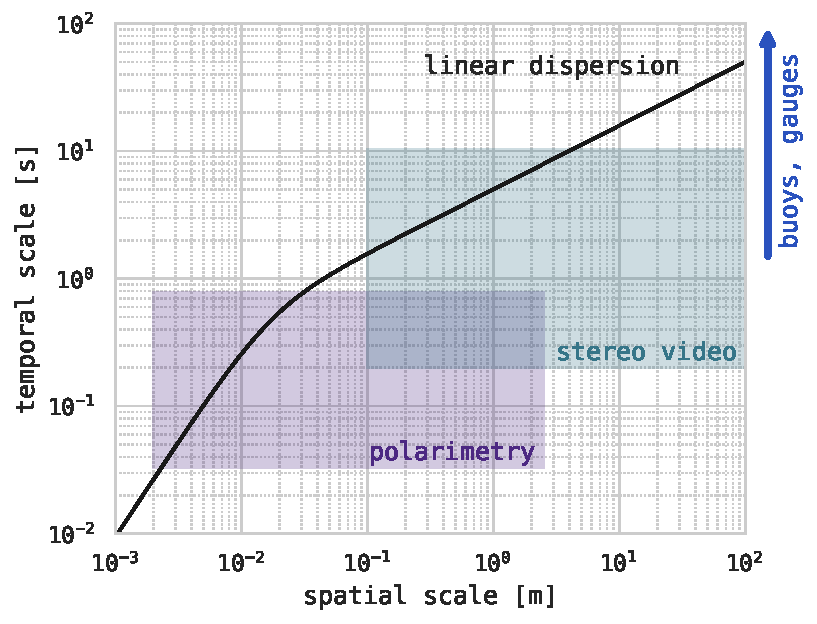
\includegraphics[width=\linewidth]{_figures/wave_measurement_stommel_diagram.pdf}
    \caption{Stommel diagram showing the spatiotemporal range of select wave measurement techniques: polarimetric slope sensing, stereo video, and point-like objects (buoys, fixed gauges). Note that the point-like objects provide no direct access to spatial information.}
    \label{fig:wave_measurement_stommel_diagram}
\end{figure}

The Stommel diagram shown in Figure \ref{fig:wave_measurement_stommel_diagram} compares the spatiotemporal ranges of select wave measurement techniques: PSS, stereo-video, and point-like gauges like buoys. In order to obtain a true spatiotemporal measurement of the surface wave field, it is important for the observational technique to envelop the linear dispersion relation, here provided in the black curve on Figure \ref{fig:wave_measurement_stommel_diagram}. The violet shaded region corresponding to PSS is somewhat flexible: by increasing the imaging field of view (usually, through increasing the freeboard above the mean sea surface), one may shift the region to the right, therefore extending the effective maximally-resolvable temporal scale. Practitioners of wave-sensing stereophotogrammetry have extended the effective temporal window of the technique through time series analysis; e.g., Benetazzo \emph{et al.} [2018] \cite{Benetazzo2018} employed the maximum entropy method (MEM) technique \cite{lygre_maximum_1986} to their surface elevation and slope estimates to infer the frequency-directional spectra of waves larger than the stereo field of view. 

\begin{figure*}[!ht]
\centering
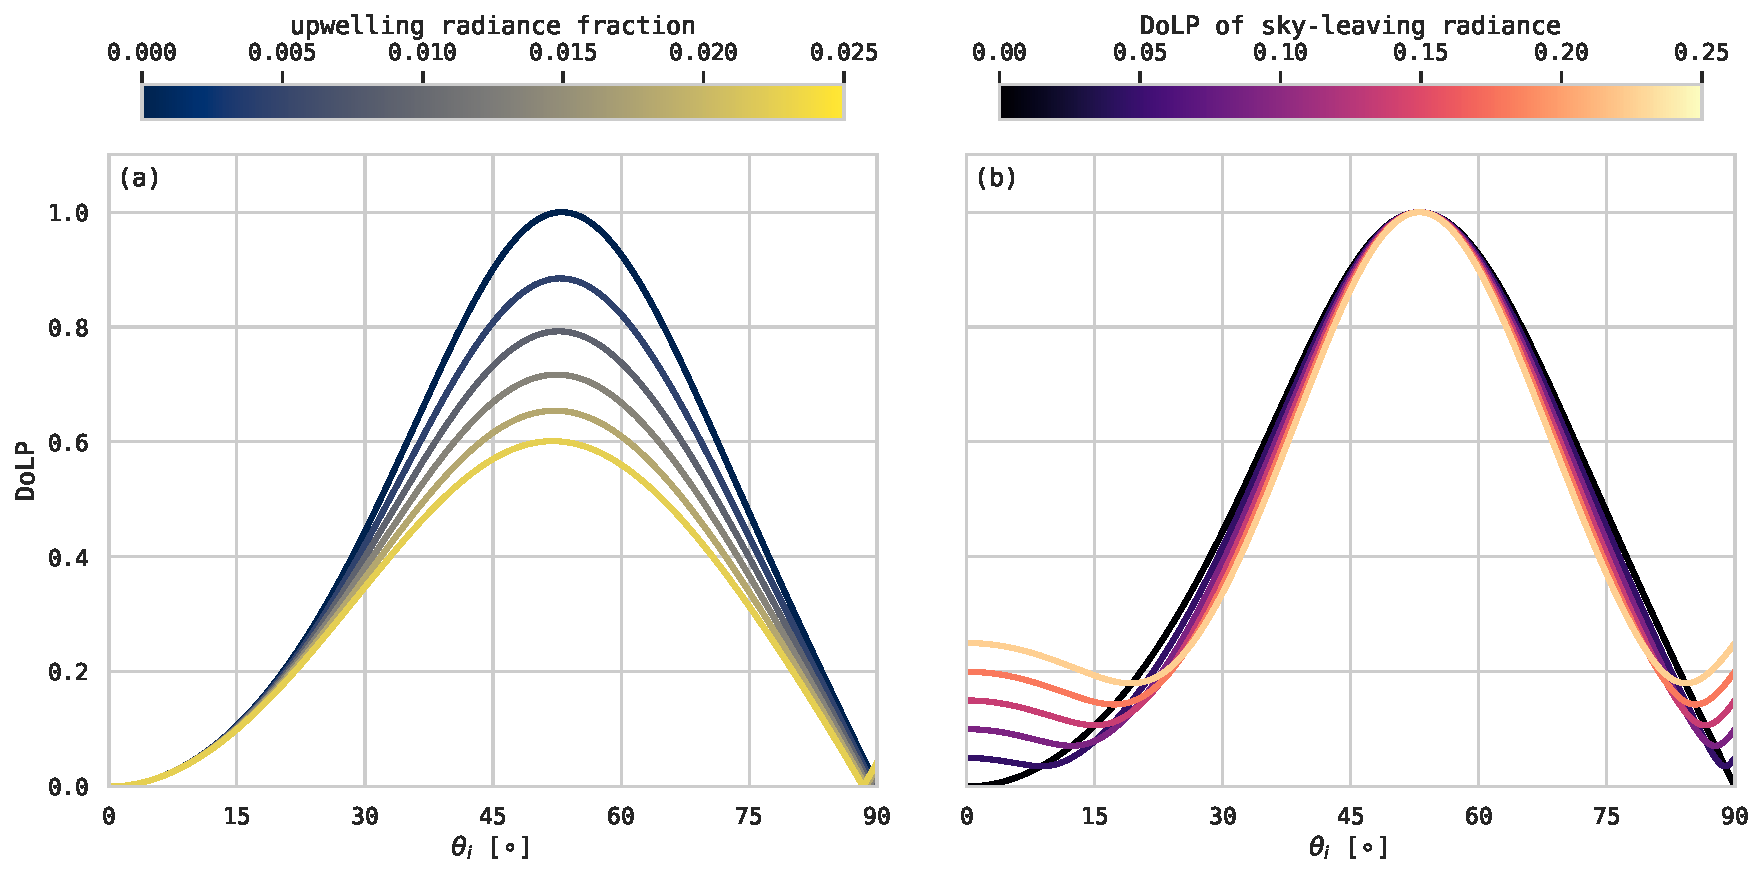
\includegraphics[width=\textwidth]{_figures/mueller_calc_example.pdf}
\vspace{-20pt}
\caption{Relationships between incidence angle ($\theta_i$) and degree of linear polarization (DoLP) given variations in \textbf{(a)} fraction of received radiance which is upwelling and \textbf{(b)} DoLP of sky-leaving radiance.}
\label{fig:mueller_calc_example}
\end{figure*}

\section{Methodology}
\label{sec:methodology}

The central assumption baked into the single-camera application of PSS is that sky-leaving radiance is unpolarized and upwelling (surface-leaving, but scattered from below the interface) radiance is negligible. This allows one to constrain the relationship between a measurement of degree of linear polarization (DoLP) and the incidence angle ($\theta_i$) of the light ray. In practice, however, even small variations in ambient environmental conditions can have a significant impact on the relationship between the measured degree of linear polarization and the incidence angle that one might infer \cite{goldstein_polarized_2017,voss_polarized_1997}. In Figure \ref{fig:mueller_calc_example}(a), we show that even a small fraction of radiance which is upwelling and unpolarized can have a significant impact in compressing the DoLP that would be measured by an imaging polarimeter. Conversely, as shown in Figure \ref{fig:mueller_calc_example}(b), the effect of polarized sky-leaving radiance is to raise the floor of the variation of DoLP across all values of $\theta_i$. The combined effect of variable sky-leaving and surface-leaving radiance is to modify this relationship. One approach to solving this problem might be to triple the number of imagers, including in one's sensing suite a floating polarimeter for obtaining upwelling light measurements and a sky-oriented polarimeter for obtaining downwelling light measurements. This would allow one to incorporate these measured values into the Fresnel reflection coefficients and directly compute the relationship between DoLP and $\theta_i$ following Mueller calculus. However, one of the greatest benefits of polarimetric slope sensing is that it requires a single camera with no in-water component and no sky-looking camera. Adding additional requirements for in-water recovery of light polarization and sky-looking state would render the technique somewhat esoteric and limit it to specialists in the field of environmental optics. Another approach might be to have two cameras but rather than have one look at the sky and one at the surface we make a measurement of our slope field with a narrow field of view lens and have a second camera alongside it to make a direct measurement of the relationship between degree of linear polarization and incidence angle with a wide format lens. This direct measurement of DoLP($\theta_i$) would natively account for the sky leaving, the polarization state of sky leaving radiance and the fraction of light which comes up through the surfaced unpolarized. Furthermore, it would also implicitly account for path losses to the polarization state, making it an attractive option for airborne applications of polarimetric slope sensing. We will address the viability of that two-camera approach later in the manuscript. For now, we focus on attempting to solve our problem with a single downward-looking, narrow field of view camera, setting the task before us to correct for unpolarized upwelling radiance and polarized sky leaving radiance in a way that is robust, flexible, and does not depend on having multiple in water and sky looking imaging polarimeters.

\begin{figure*}[!ht]
    \centering
    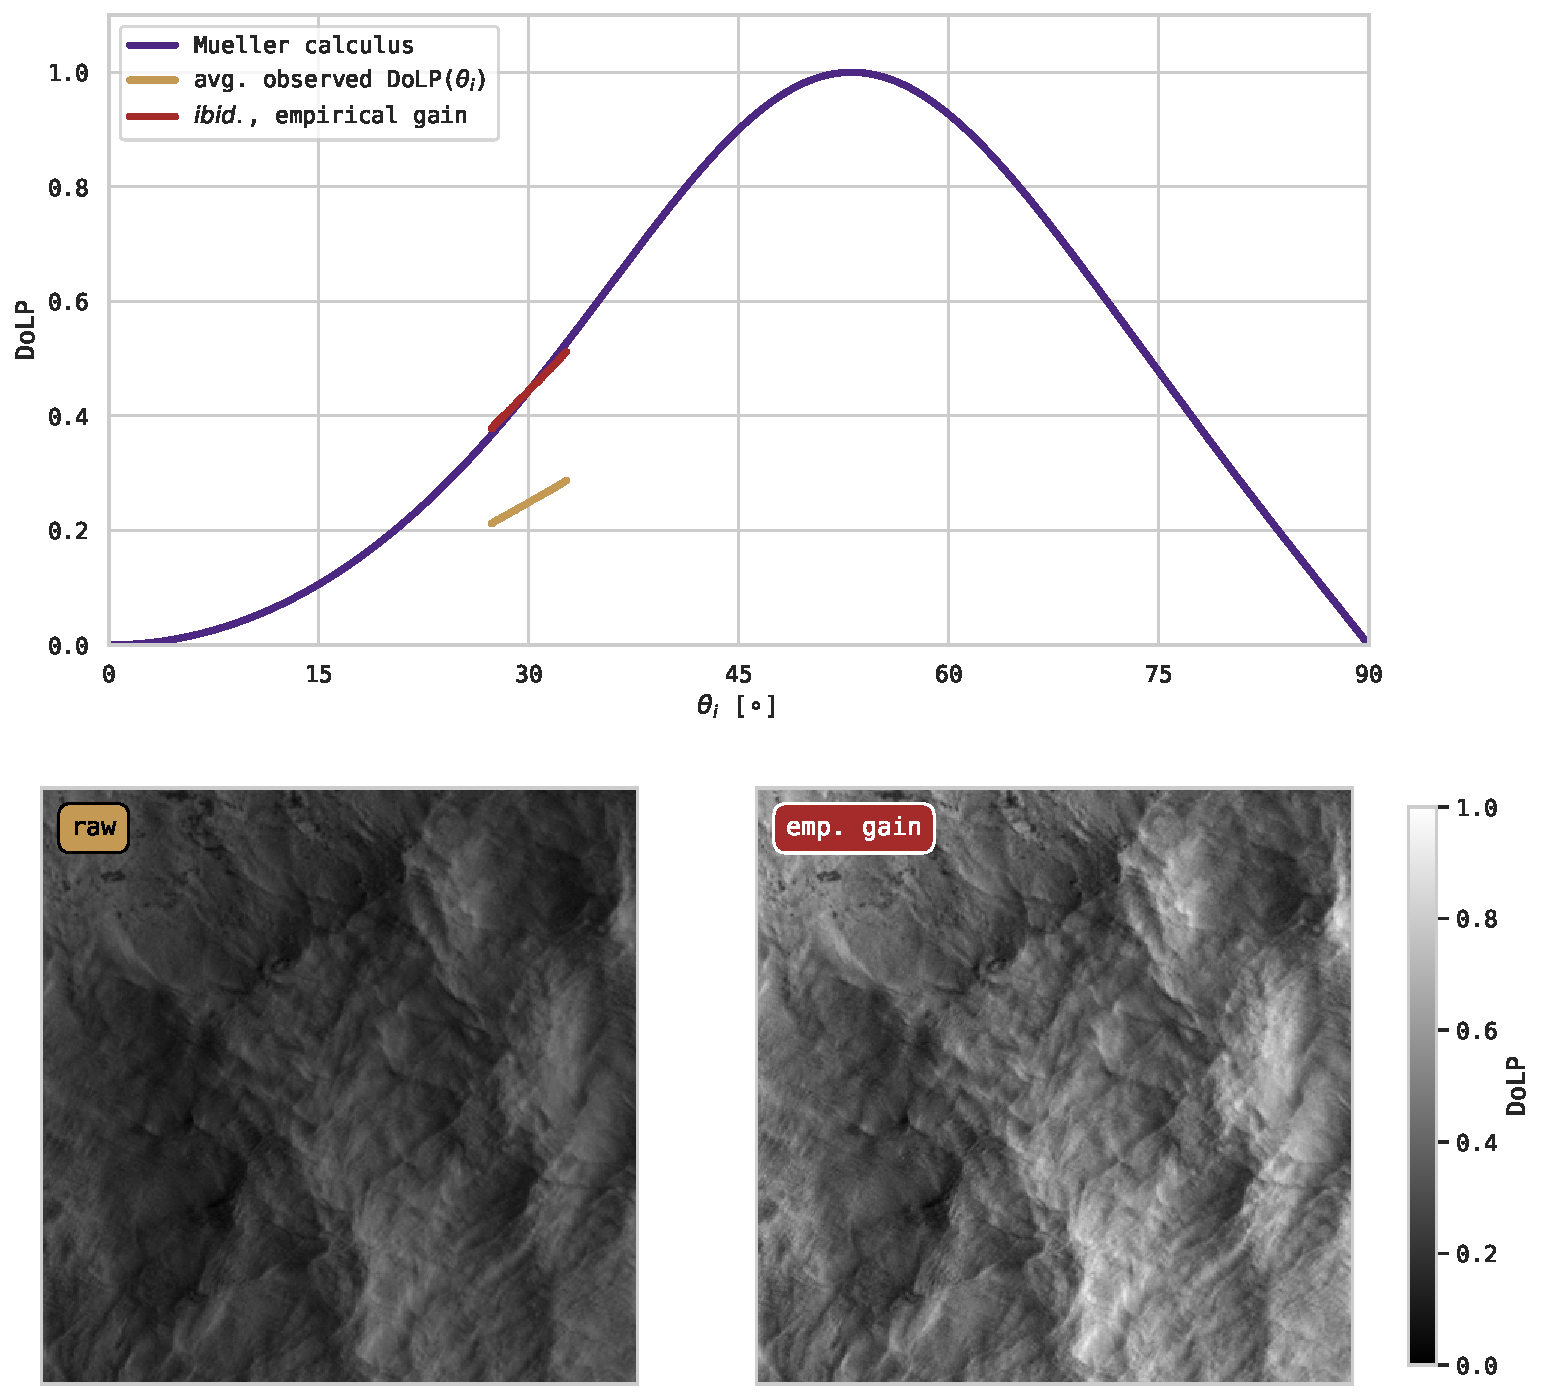
\includegraphics[width=\textwidth]{_figures/DoLP_AOI_gain_example.pdf}
    \vspace{-20pt}
\caption{Top: variation of degree of linear polarization (DoLP) with incidence angle ($\theta_i$) as computed through Mueller calculus or observed via polarimetric camera. Bottom: spatial variation of DoLP provided no gain or an empirical gain.}
\vspace{-15pt}
\label{fig:DoLP_AOI_gain_example}
\end{figure*}

\newpage

Even under pristine laboratory conditions, a polarimeter may not perform ideally (that is, show ideal response when subjected to an integrating sphere/rotating linear polarizer test). This may be due to a number of factors, among them depolarization of light by optics or deviation of the sensor from optimal sensitivity. Correcting for these persistent effects is essential to making a good measurement \cite{Zappa2012,Laxague2018b,laxague_suppression_2024,laxague_effects_2025}. During integrating sphere polarizer tests of our DoFP detector, we found the normalized Stokes parameter amplitude to be 0.81 (rather than the ideal 1.0). The difference between $S_1$ and $S_2$ amplitudes was determined to not be statistically significant ($p=0.74$, $N=12$). We found the mean Stokes parameter to be slightly variable around zero (rms$\approx$5\%) with a directional asymmetry between minima and maxima of the Stokes parameters on the order of 2-3\% of the amplitude.

This calibration is an important first step, though it will not account for variability in the ambient illumination conditions. We demonstrate an empirical approach to accounting for variability in upwelling/downwelling radiance in Figure \ref{fig:DoLP_AOI_gain_example}. The violet curve in the top panel represents the relationship between DoLP and $\theta_i$ which would arise due to unpolarized sky living radiance and no upwelling radiance (that is, the most simple form of Mueller calculus). The gold segment on that panel correseponds to the observed variation of DoLP from the bottom to the top of the image frame as averaged over a single ten-minute period. The range of $\theta_i$ is obtained directly from the known mounting geometry of the instrument and the vertical angle of view for the camera-lens combination (here 30$^{\circ}\pm$2.7$^{\circ}$ for a 75 mm lens).

\begin{figure*}[!ht]
    \centering
    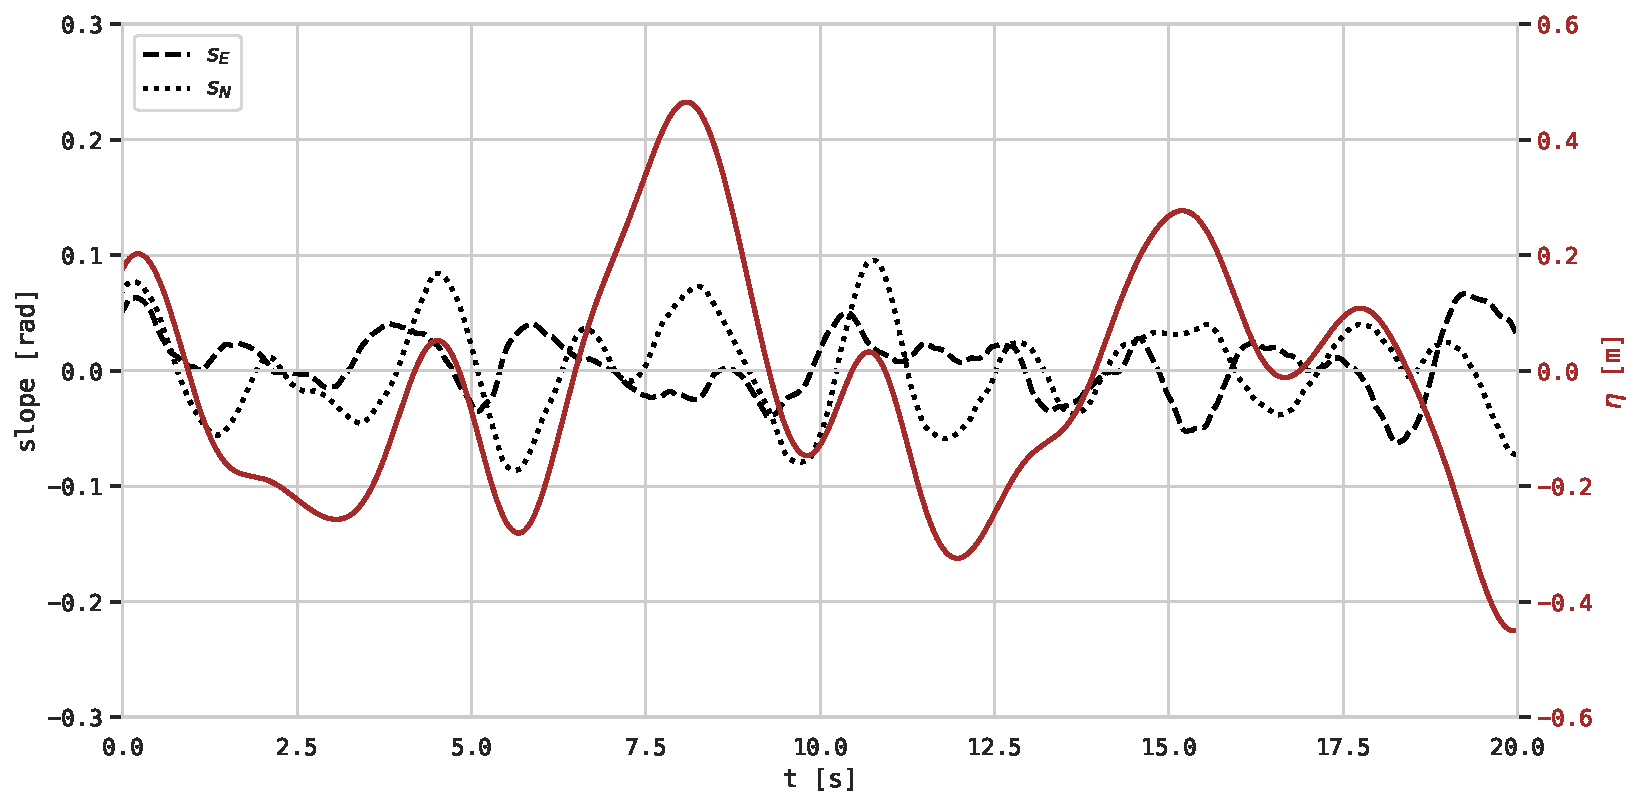
\includegraphics[width=\textwidth]{_figures/wave_slope_elev_timeseries.pdf}
    \vspace{-20pt}
\caption{Temporal variation of east and north wave slope ($s_E$ \& $s_N$, respectively) along with the corresponding water surface elevation $\eta$ computed via the Fourier space inversion approach of equation \ref{eq:slope_inversion}.}
\vspace{-15pt}
\label{fig:wave_slope_elev_timeseries}
\end{figure*}

A corresponding snapshot of the full-frame DoLP is given in the bottom left panel, marked with a label of \lq\lq raw". The \emph{empirical} gain is simply the value by which the frame-median DoLP needs to be scaled in order to yield the value expected for zero upwelling radiance and unpolarized sky-leaving radiance. After application of the empirical gain to the time-averaged DoLP, we obtain the red segment in the top panel. When that gain value is applied to the DoLP snapshot, we obtain the field shown in the bottom right panel.

Absent supporting independent information regarding upwelling and sky-leaving radiance, this empirical approach seems to be the most straightforward: the known orientation of the camera defines the slope reference on a case-by-case basis. Nevertheless, it is important that we demonstrate the positive impact of this approach. The best way to accomplish this would be to have a secondary measurement that could act as a gold standard; however, the principal benefit of PSS is that it is the sole established technique for field observations of short to intermediate-scale ocean waves. During the Fall and Winter of 2019-2020, a set of targeted measurements of wind forcing, surface waves, and near-surface currents were made at the Air-Sea Interaction Tower (ASIT) just south of Martha's Vineyard, MA \cite{laxague_effects_2025}. As part of this campaign (hereinafter \lq\lq ASIT2019"), we obtained wind speed and turbulent fluxes along with the water surface elevation time series via near-infrared LiDAR. For some observational cases, we also obtained the frequency-directional wave spectrum via bottom-mounted ADCP. In order to demonstrate the efficacy of the empirical gain approach, we will compare the wave height and mean wave period obtained via LiDAR measurements to the same quantities inferred from surface slope field measurements.

The first step in this comparison is to infer the water surface elevation time series from the time series of two-component surface slope, as in equation \ref{eq:slope_inversion}:
\begin{align}
    \label{eq:slope_inversion}
    \eta(t)=\mathcal{F}^{-1}\Big\{-\frac{i}{k}\Big[\mathcal{F}\{s_E\}+\mathcal{F}\{s_N\}\Big]\Big\}
\end{align}

\newpage

This inversion follows directly from small-amplitude (linear) water wave theory. It is analogous to orbital velocity/pressure inversion techniques \cite{guza_local_1980}, and can be thought of as a one-dimensional application of the slope field inversion technique of Frankot \& Chellappa \cite{Frankot1988}. A demonstration of this approach is presented in Figure \ref{fig:wave_slope_elev_timeseries}. The east and north oriented slope components are provided as dashed and dotted curves, respectively, while the red trace indicates the resulting water surface elevation time series $\eta$ inferred from the slope time series. The corresponding omnidirectional frequency spectra are provided in Figure \ref{fig:elevation_omnispect}. Note that the frame size of $L\approx$ 3 m limits the proper frequency response above 0.35 Hz (wavelength $\approx$ $4L$).

\begin{figure}[!ht]
    \centering
    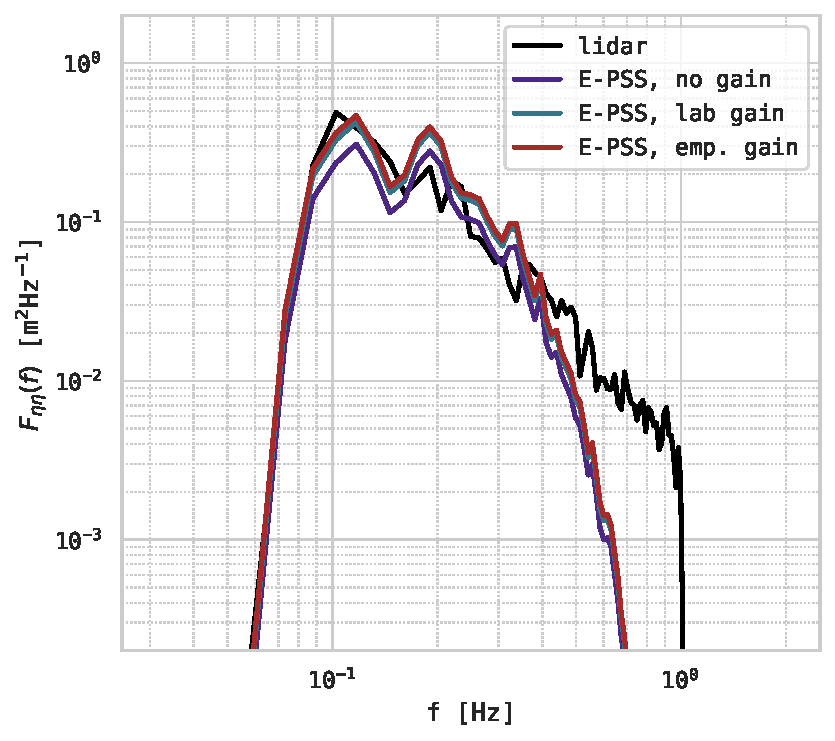
\includegraphics[width=0.49\textwidth]{_figures/elevation_omnispect.pdf}
    \vspace{-25pt}
\caption{Omnidirectional spectra computed from water surface elevation timeseries obtained by LiDAR and E-PSS.}
\label{fig:elevation_omnispect}
\end{figure}

\newpage

\section{Results}
\label{sec:results}

From this point forward, we use the acronym E-PSS (Extended Polarimetric Slope Sensing) to describe a combination of (1) polarimetric slope sensing with a laboratory or empirically-based modification to the DoLP($\theta_i$) relationship and (2) the estimation of surface elevation via Fourier space inversion of the slope time series. As shown in Figure \ref{fig:mueller_calc_example}b, unpolarized sky-laving radiance will elevate the lowest degree of linear polarization that will be observed from a downward-looking imaging polarimeter. However, we did not find there be an elevated floor the measurements of DoLP made over a range of ambient conditions (full sun to full overcast) during the 2019-2020 ASIT field campaign. To be specific, we found frequent occurrence of low ($<$0.1) values of DoLP for all ambient illumination conditions, indicating that variability in sky-leaving polarization state is likely to be of secondary importance for PSS. However, given the somewhat large values of empirical DoLP gain (1.2-1.7) used during our field observations, upwelling radiance should not be neglected. This is consistent with previous studies of upwelling radiance \cite{You2011,ibrahim_relationship_2012}. Based on the values provided in Figure \ref{fig:mueller_calc_example}a, it's reasonable to expect that between 1-3\% of the radiance received by our imaging polarimeter is unpolarized, upwelling radiance that is diluting the measurement that we would be making from surface reflected light. This would indicate that an approach which allows for a variable gain (e.g., our empirical approach) to have a significant advantage over the static laboratory-based calibration.

The benefit of using an empirical gain approach is demonstrated in the scatter plot of Figure \ref{fig:Hm0_comparison_lidar_epss}, wherein we compare the significant wave height computed from LiDAR and E-PSS-derived wave spectra. We compute the significant wave height as four times the square root of the zeroth moment of the wave spectrum, $H_{m0}=4\times\Big(\int_0^\infty F(f)~\mathrm{d}f\Big)^{1/2}$.

\begin{figure}[!ht]
    \centering
    \includegraphics[width=0.49\textwidth]{_figures/Hm0_comparison_lidar_epss.pdf}
    \vspace{-20pt}
    \caption{Scatterplot comparing significant wave height ($H_{m0}$) estimates from lidar and E-PSS for each of the three DoLP gain values. Dots mark individual observations while lines represent the least-squares linear fits (with shaded regions demarcating 95\% confidence intervals). Key error metrics (computed with respect to $H_{m0}$, lidar) are given in the figure legend.}
    \vspace{-10pt}
    \label{fig:Hm0_comparison_lidar_epss}
\end{figure}

The figure legend contains pieces of key statistical information about the comparison between LiDAR and E-PSS estimates. The no-gain and laboratory-gain approaches provide significant wave heights which are substantially lower than those produced from the LiDAR measurements. However, the $H_{m0}$ estimates produced via empirical gain approach are appropriately close to those obtained by LiDAR: $R^2\approx$ 0.76, RMSE $\approx$ 32 cm, and a fit slope of 0.98, indicating nearly one-to-one response.
An analogous comparison is provided in Figure \ref{fig:Tm02_comparison_lidar_epss}, where we show the mean wave period computed both from LIDAR and E-PSS measurements. The mean wave period ($T_{m02}$) is defined in the following manner:
\begin{align}
    T_{m02}\equiv\Big(\frac{m0}{m2}\Big)^{1/2}=~ \Bigg(\frac{\int_0^\infty F(f)~\mathrm{d}f}{\int_0^\infty f^2F(f)~\mathrm{d}f}\Bigg)^{1/2}
\end{align}

Note that the E-PSS estimate of $T_{m02}$ is less sensitive than $H_{m0}$ to the DoLP gain value: the frequency response is weakly sensitive to the choice of gain, whereas the total energy contained within the spectrum is quite sensitive to the gain. The underestimation of $T_{m02}$ by E-PSS for moderate to long wave periods is likely due to the method's performance at low frequencies. The Fourier space transfer function between slope and surface elevation goes like $k^{-1}\propto f^{-2}$, requiring a somewhat aggressive highpass filter to curtail spuriously-high energy at low frequencies. We established a passband of 0.08 Hz $\le f \le$ 1 Hz; however, application of a lowpass filter is somewhat redundant due to the spatial averaging inherent to the process of computing the mean slope over our 2.5 m $\times$ 2.5 m field of view ($f_{cut}\approx$ 0.75 Hz).

\begin{figure}[!ht]
    \centering
    \includegraphics[width=0.49\textwidth]{_figures/Tm02_comparison_lidar_epss.pdf}
    \vspace{-20pt}
    \caption{Analogue to Figure \ref{fig:Tm02_comparison_lidar_epss} for mean wave period ($T_{m02}$).}
    \label{fig:Tm02_comparison_lidar_epss}
\end{figure}

\newpage

\begin{figure*}[!ht]
    \centering
    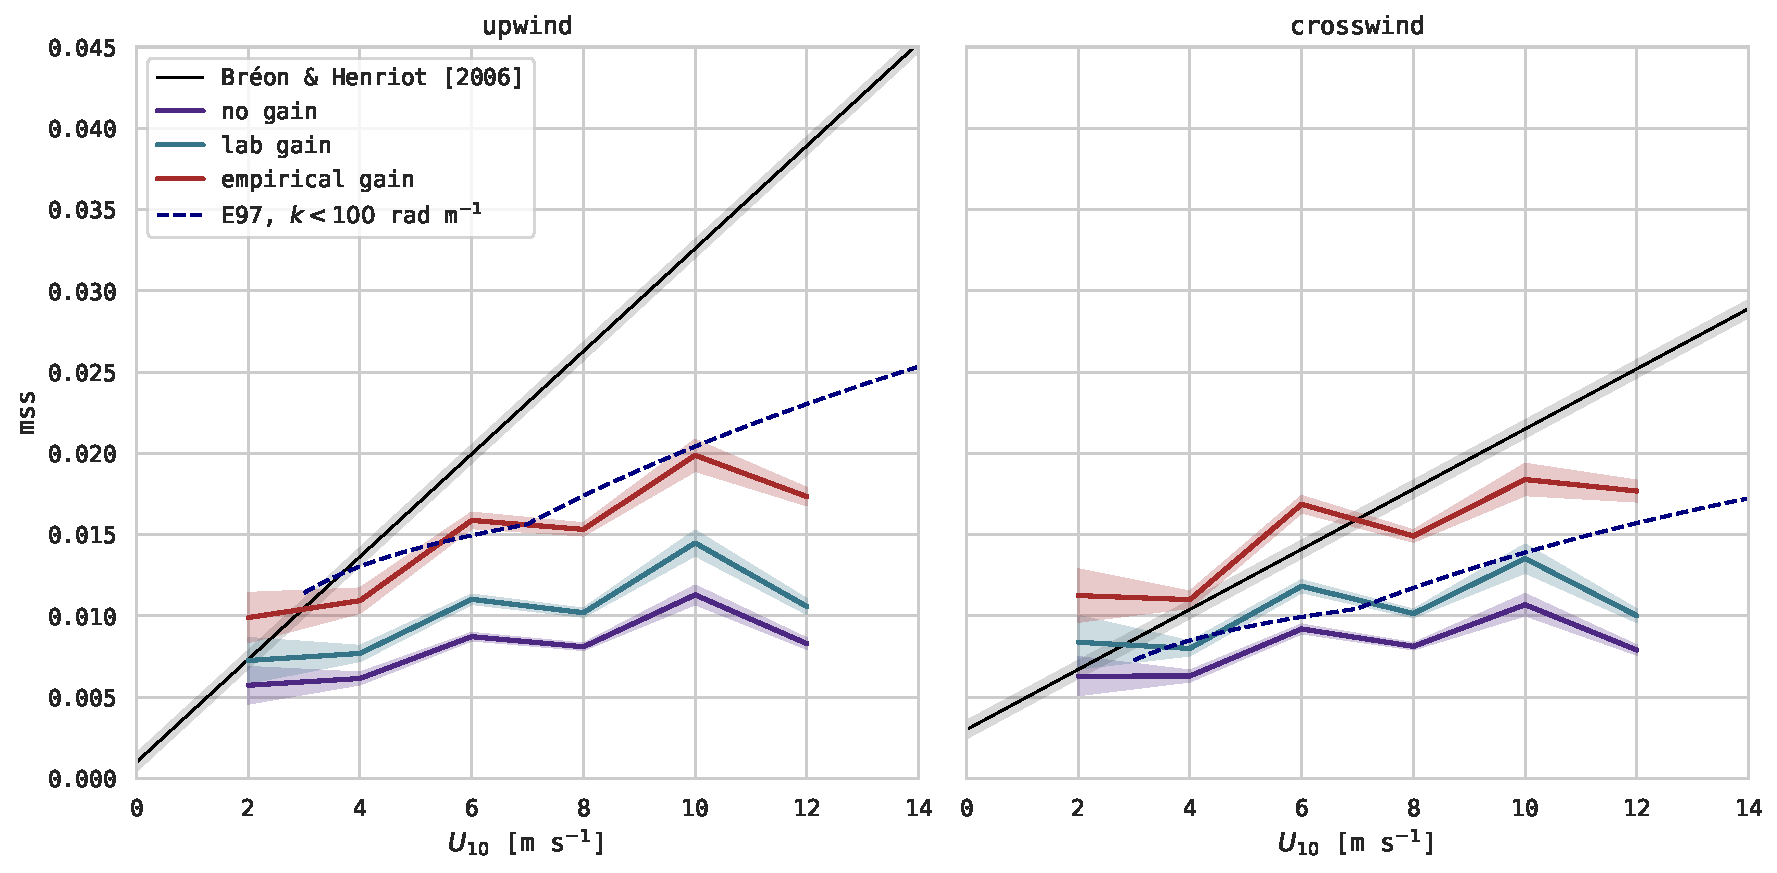
\includegraphics[width=\textwidth]{_figures/mss_upwind_crosswind.pdf}
    \vspace{-20pt}
    \caption{Upwind and crosswind mean square slope computed from wave slope fields given the three modes of DoLP gain application. Shaded regions demarcate the 95\% confidence interval about the mean. Black lines and shaded regions represent the least-squares fits and uncertainties of Br\'eon \& Henriot [2006]. The dashed blue trace marks values of $mss$ computed from the spectrum of Elfouhaily \emph{et al.} [1997] \cite{Elfouhaily1997} assuming a high wavenumber cutoff of 100 rad m$^{-1}$.}
    \label{fig:mss_upwind_crosswind}
    \vspace{-10pt}
\end{figure*}

The joint probability density function (PDF) for upwind and crosswind wave slope is approximately Gaussian. In the real ocean, wind stress and long surface waves impact the short wave slope distribution in a way that yields non-zero skewness and kurtosis (peakedness). Cox \& Munk [1954] accounted for this by providing a Gram-Charlier polynomial expansion about a Gaussian distribution \cite{Cox1954a}, here provided in equation \ref{eq:gram-charlier}:
\begin{align}\label{eq:gram-charlier}
\begin{split}
P(\xi,\zeta)
  &= \frac{1}{2\pi\sigma_{up}\sigma_{cr}}\mathrm{exp}\Big(-\frac{\xi^2+\zeta^2}{2}\Big)          \\[6pt]
  &\quad\hfill
     \cdot\left\{
     \begin{aligned}
       1 &- \frac{1}{2}c_{21}(\xi^2-1)\zeta\\
       &- \frac{1}{6}c_{03}(\zeta^3-3\zeta)\\
       &+ \frac{1}{24}c_{40}(\xi^4-6\xi^2+3)\\
       &+ \frac{1}{24}c_{04}(\zeta^4-6\zeta^2+3)\\
       &+ \frac{1}{4}c_{22}(\xi^2-1)(\zeta^2-1)\\
       &\quad\vdots
     \end{aligned}
     \right\}
\end{split}
\end{align}

We omit the expansion's higher-order terms. The quantities $\sigma_{up}$ and $\sigma_{cr}$ correspond to the standard deviations about the mean of upwind and crosswind slopes, respectively. The independent variables of the distribution, $\xi$ and $\zeta$, represent the crosswind and upwind wave slopes normalized by the corresponding wave slope standard deviation.

The variation of upwind and crosswind mean square slope (i.e., $\sigma_{up}^2$ and $\sigma_{cr}^2$, respectively) with ten-meter wind speed $U_{10}$ observed during ASIT2019 is provided in Figure \ref{fig:mss_upwind_crosswind}. The three different colored segments indicate measurements of mean square slope obtained from E-PSS given the three aforementioned DoLP gain modes (no gain, laboratory-derived gain, empirical gain). Shaded regions on the three colored curves from our measurements correspond to 95\% confidence intervals about the mean. The black line marks the results of Br\'eon \& Henriot [2006] \cite{Breon2006} which are in close agreement with the classic Cox \& Munk [1954] \cite{Cox1954a} observations. The shaded region about the black lines correspond to Br\'eon \& Henriot's reported level of uncertainty. The blue dashed trace represents upwind/crosswind slope variance computed from the wavenumber-directional spectrum of Elfouhaily \emph{et al.} [1997] \cite{Elfouhaily1997} assuming a high wavenumber cutoff of 100 rad m$^{-1}$.

The joint PDF for upwind and crosswind wave slope was computed for all ASIT2019 observational cases with the three aforementioned DoLP gain modes. From these we obtained the marginal PDFs: the upwind slope PDF and the crosswind slope PDF. A selection of these (bin-averaged by ten-meter wind speed $U_{10}$) are shown alongside the Br\'eon \& Henriot [2006] \cite{Breon2006} marginal PDFs in Figure \ref{fig:slope_distributions_binned_by_wind}. We performed a least-squares fit to each wave slope joint PDF, specifying the functional form as the Gram-Charlier expansion of a Gaussian (equation \ref{eq:gram-charlier}). This exercise yielded the coefficients $c_{21}$ \& $c_{03}$ (correseponding to skewness) and $c_{40}$, $c_{04}$, \& $c_{22}$ (corresponding to kurtosis). We present these coefficients in Figure \ref{fig:slope_distribution_GC_coeffs}, bin-averaged by ten-meter wind speed $U_{10}$ and shown alongside the results of Br\'eon \& Henriot [2006] \cite{Breon2006} and Cox \& Munk [1954] \cite{Cox1954a}. Colored segments correspond to the results of E-PSS, with shaded regions representing the 95\% confidence interval about the mean. The shaded regions around the black traces of Br\'eon \& Henriot correspond to their empirically derived levels of uncertainty. In panel (f) we provide the number of samples per wind speed bin ranging from 10 to 40 per wind speed bin.

\begin{figure*}[!ht]
    \centering
    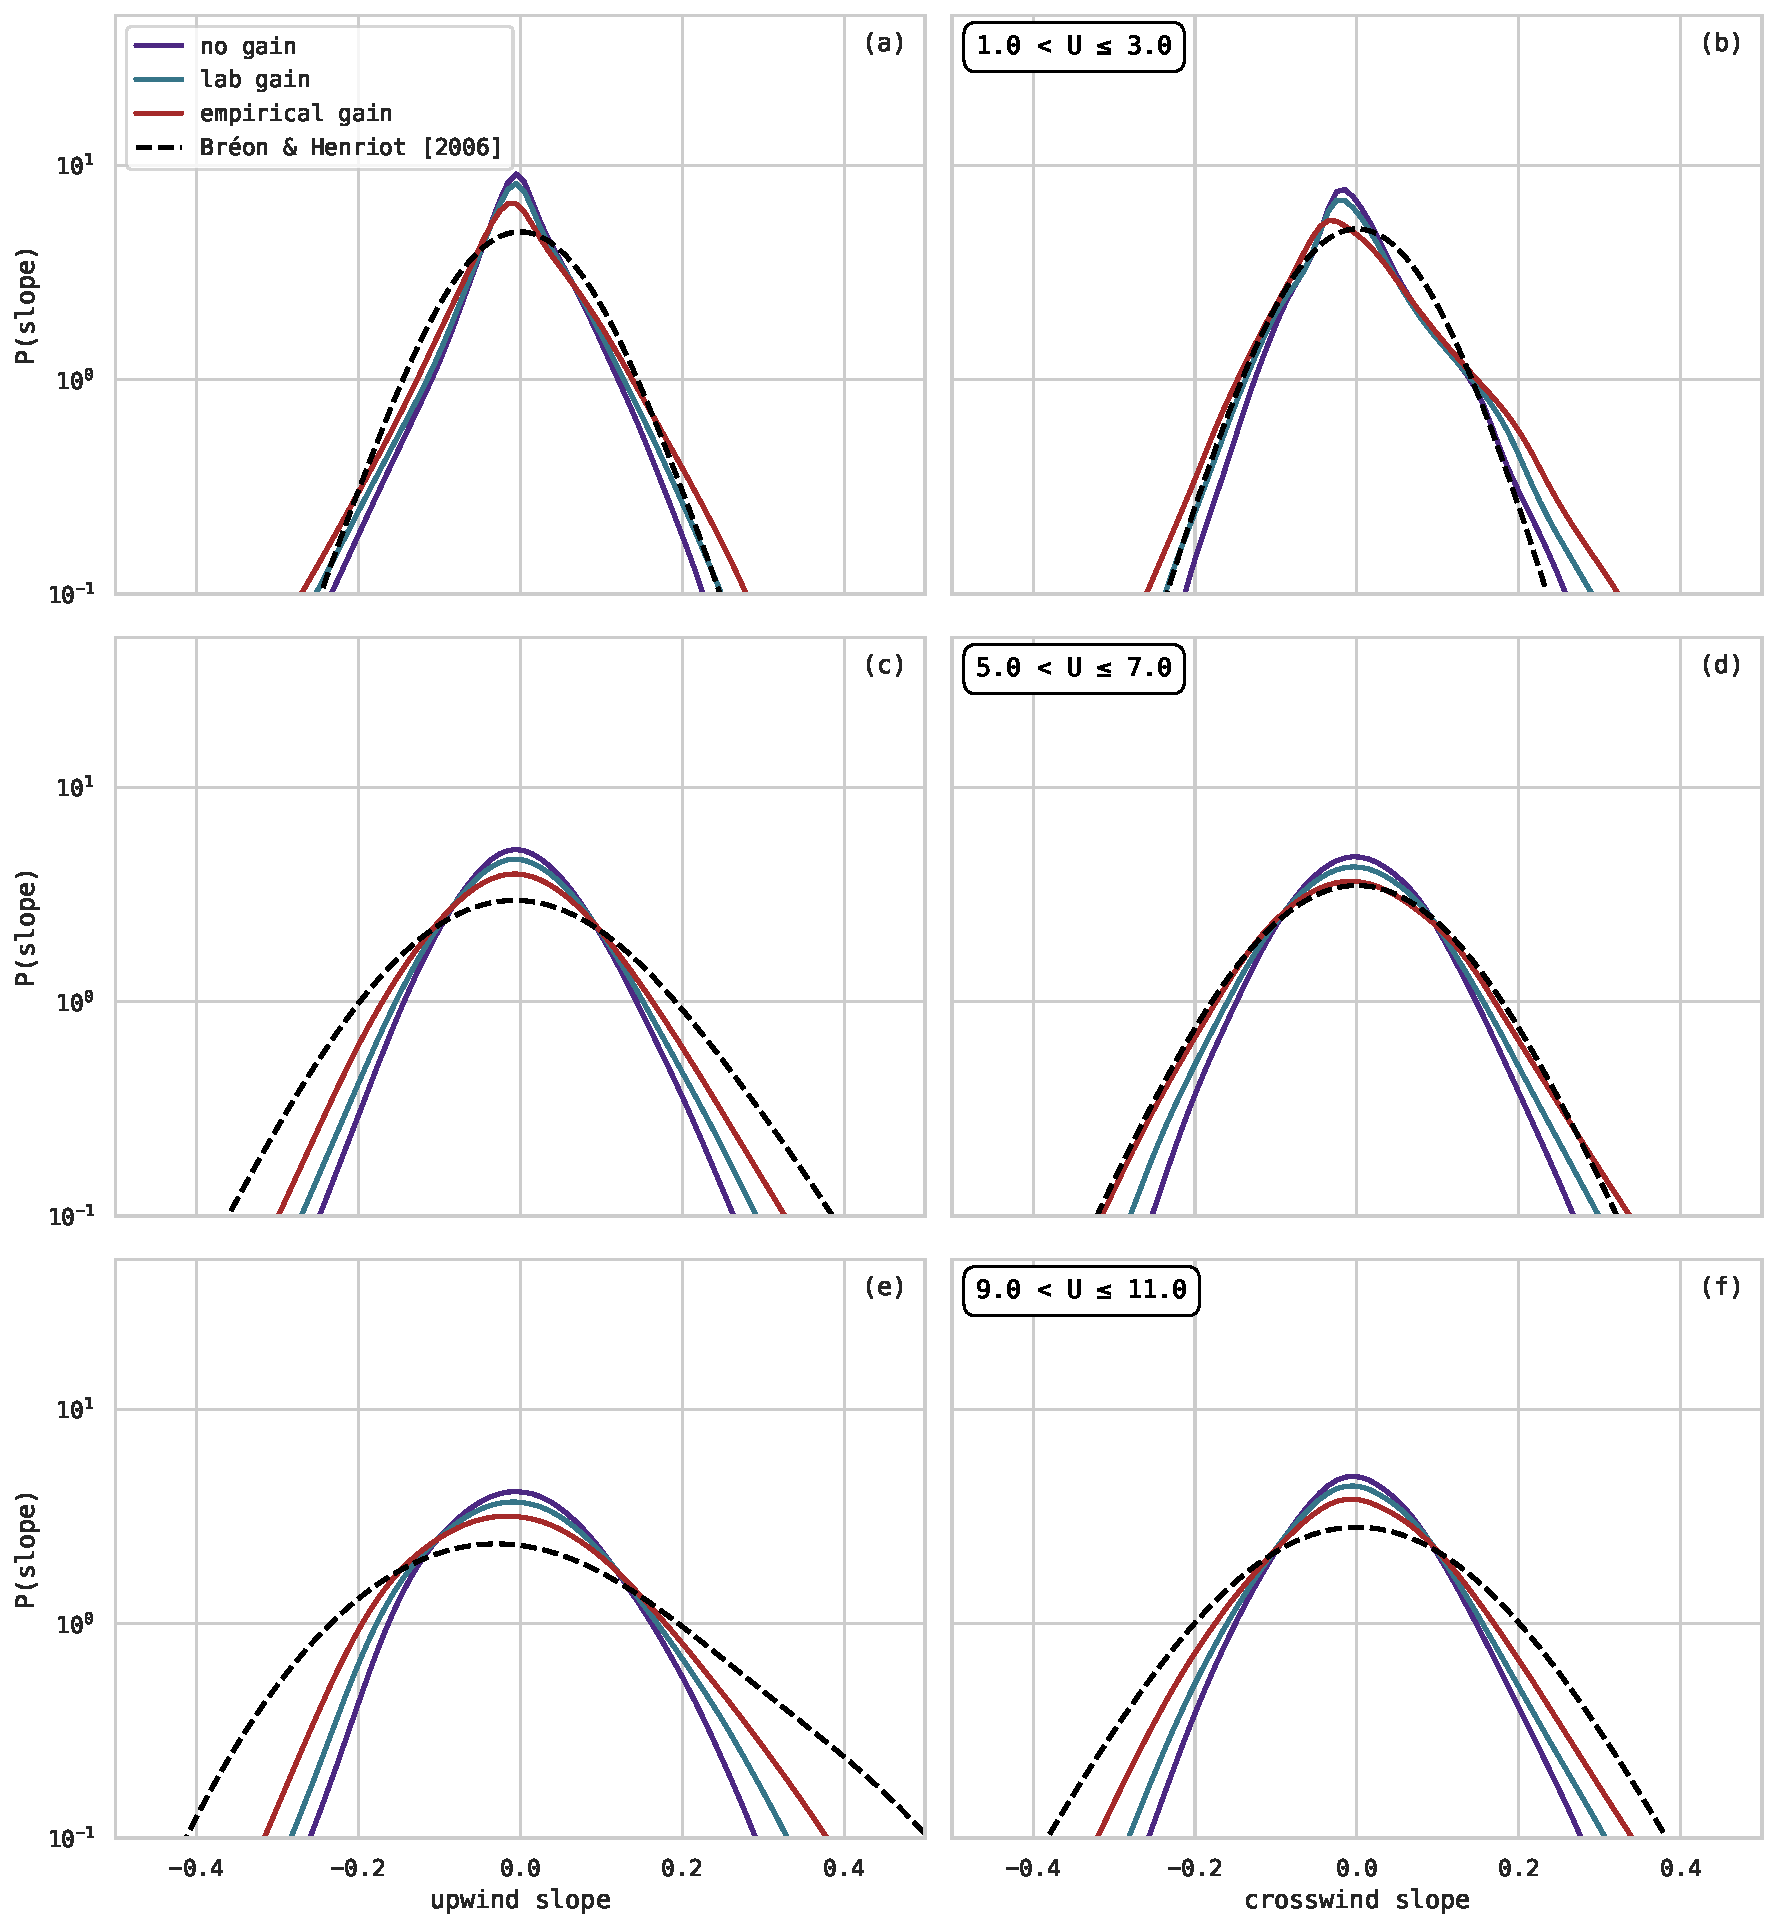
\includegraphics[width=\textwidth]{_figures/slope_distributions_binned_by_wind.pdf}
    \vspace{-20pt}
\caption{Slope probability density functions, upwind (a,c,e) and crosswind (b,d,f). Colored traces correspond to PDFs produced from field observations with varying DoLP gain values. Black dashed traces correspond to Gram-Charlier distribution with coefficients taken from Br\'eon \& Henriot [2006].}
\label{fig:slope_distributions_binned_by_wind}
\end{figure*}

\begin{figure*}[!ht]
    \centering
    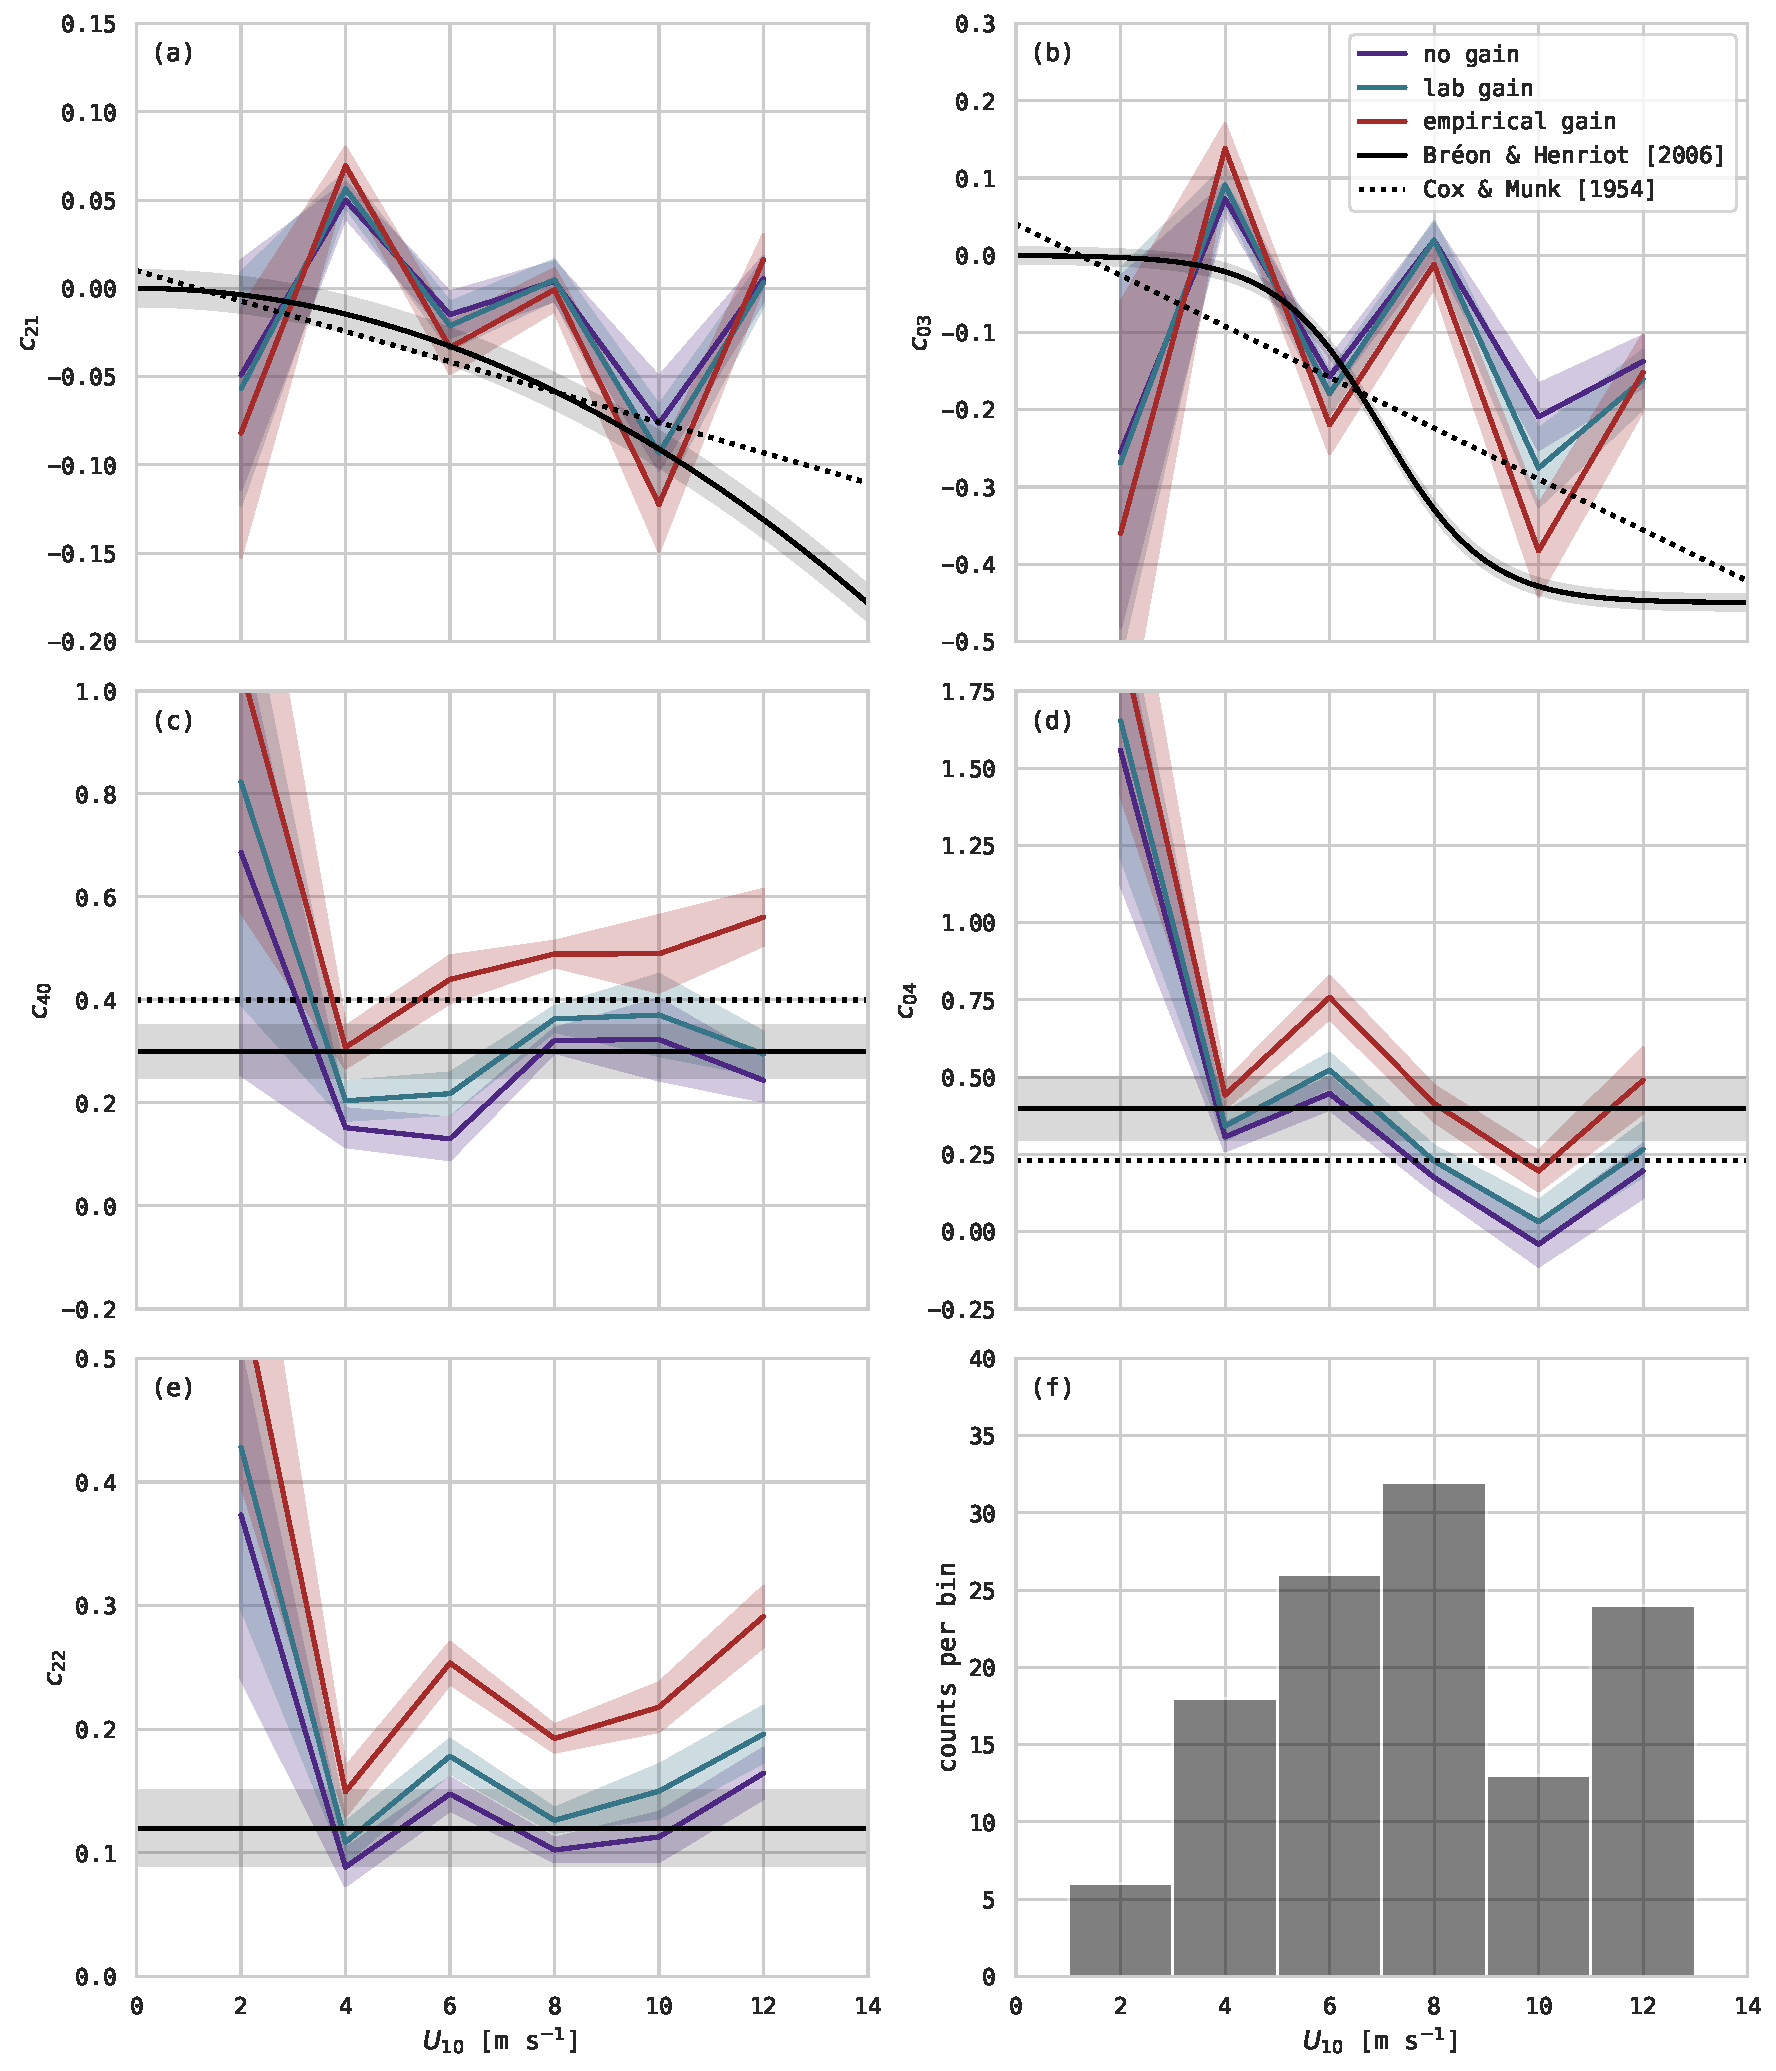
\includegraphics[width=\textwidth]{_figures/slope_distribution_GC_coeffs.pdf}
    \vspace{-20pt}
\caption{Coefficients $c_{ij}$ of the Gram-Charlier expansion to the 2D Gaussian wave slope distribution. Coefficients correspond to skewness ($c_{21}$ \& $c_{03}$) and kurtosis ($c_{40}$, $c_{04}$, \& $c_{22}$) of the distribution. Colored traces represent values averaged in bins equally-spaced in wind speed, with shaded regions marking the 95\% confidence interval about the mean. Black curves represent least-squares fits from Br\'eon \& Henriot [2006], with shaded region marking the qualitatively-determined uncertainty \cite{Breon2006}. Bar chart in panel (f) displays sample size per wind speed bin.}
\label{fig:slope_distribution_GC_coeffs}
\end{figure*}

\newpage

~\clearpage

\begin{figure*}[!ht]
    \centering
    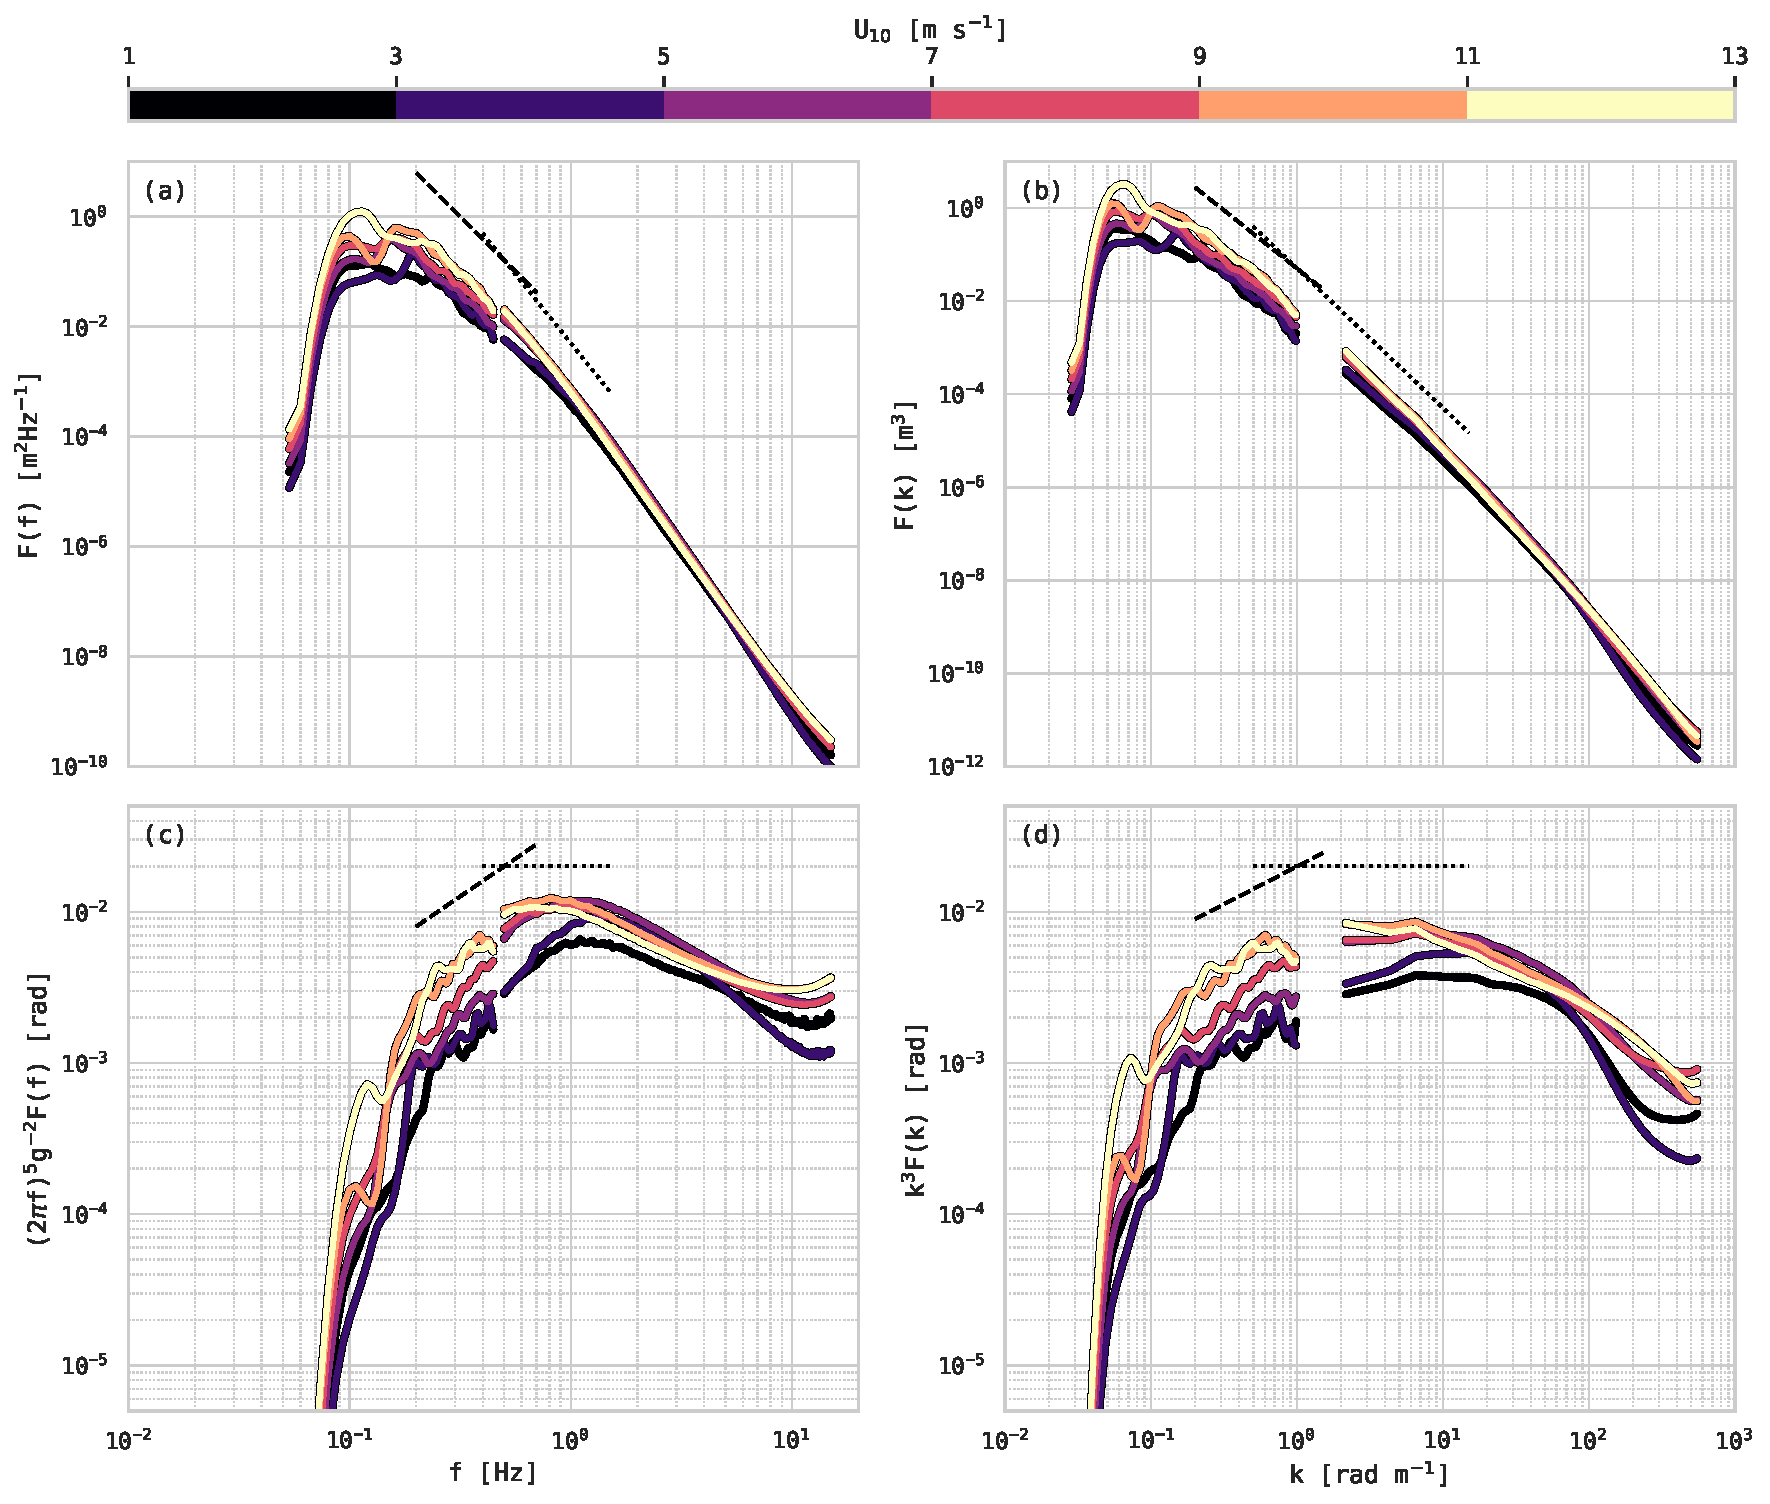
\includegraphics[width=\textwidth]{_figures/omnidirectional_spectra_binned_by_wind.pdf}
    \vspace{-20pt}
\caption{Omnidirectional spectra: (a) frequency elevation, (b) wavenumber elevation, (c) frequency saturation, (d) wavenumber saturation. Color indicates the ten-meter wind speed range for which each bin average was computed. Dashed and dotted lines correspond to power laws indicating the slope to be expected in the equilibrium ($f^{-4}$, $k^{-2.5}$ elevation; $f^{1}$, $k^{0.5}$ saturation) and saturation ($f^{-5}$, $k^{-3}$ for elevation; $f^{0}$, $k^{0}$ saturation) ranges, respectively.}
\label{fig:omnidirectional_spectra_binned_by_wind}
\end{figure*}

As demonstrated in section \ref{sec:methodology} (and shown in Figure \ref{fig:elevation_omnispect}), E-PSS allows one to infer the elevation omnidirectional frequency spectrum from the wave slope time series. We found good response for frequencies $f$ on $[0.08$ Hz, $0.5$ Hz]. For the slope field size $L^2$ of 2.91 m $\times$ 2.91 m obtained during ASIT2019, this range of frequencies corresponds to waves with wavelength $\lambda$ on $[2L, 50L]$. Polarimetric slope sensing is capable of obtaining the \lq\lq direct" wavenumber-frequency directional spectrum for waves in the range of scales constrained by the sampling rate, camera resolution, and spatial frame size. For this field campaign, the sampling rate of 30 fps and effective spatial resolution of 5.69 mm/px limited the Nyquist frequency and wavenumber to 15 Hz and 551.74 rad m$^{-1}$, respectively.

\newpage

The omnidirectional wave spectra obtained via E-PSS during ASIT2019 are shown in Figure \ref{fig:omnidirectional_spectra_binned_by_wind}. The \lq\lq direct" frequency spectra were subjected to band-averaging while the spectra produced from the inferred sea surface elevation were computed using Welch's method (one-minute non-overlapping segments, each subjected to a Hann window). Spectra have been averaged in wind speed bins of 2 m s$^{-1}$ in $U_{10}$ (as indicated by the color bar). The top row contains elevation spectra while the bottom row contains saturation spectra (i.e., compensated by $f^5$ or $k^3$). Dashed and dotted lines correspond to the equilibrium and saturation ranges, respectively. The wavenumber spectra for long waves was inferred through linear wave theory, given the water depth at ASIT of 15 meters and assuming no current.

\newpage

\begin{figure*}[!ht]
    \centering
    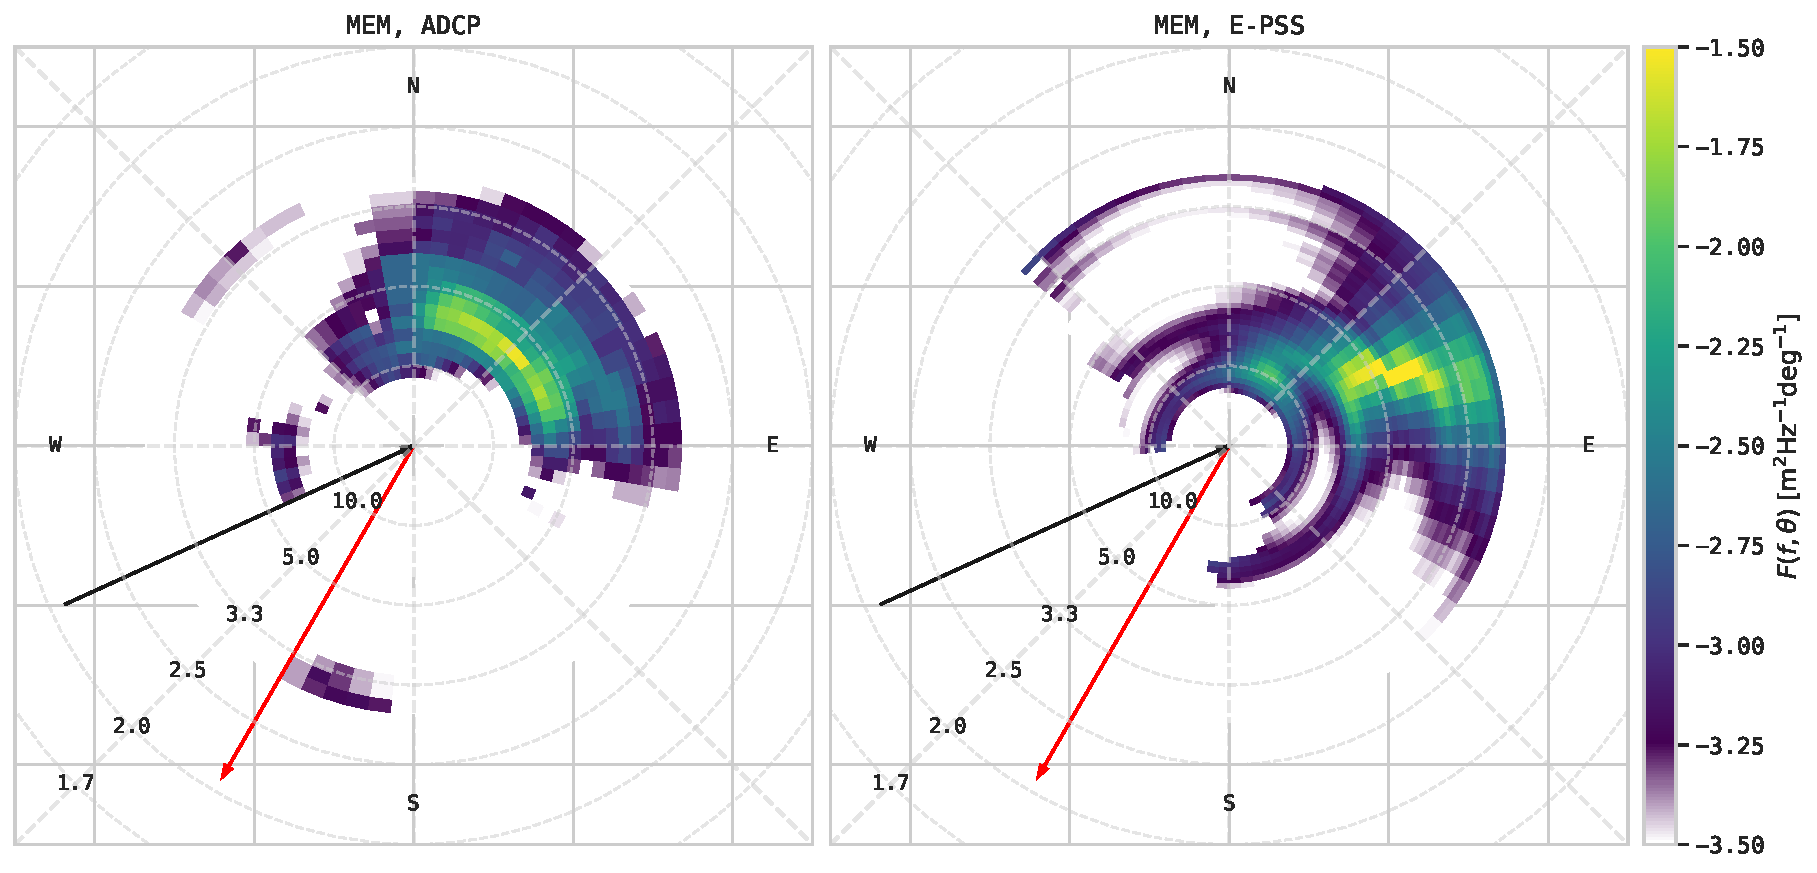
\includegraphics[width=\textwidth]{_figures/directional_spectra_polar.pdf}
    \vspace{-20pt}
\caption{Frequency-directional spectra computed via MEM given (a) the surface elevation/current profile measurements of the ADCP and (b) the measured two-component long wave slope and water surface elevation inferred via E-PSS. The black arrow indicates the wind direction ($U_{10}=$ 7.7 m s$^{-1}$) and the red arrow indicates the surface current direction ($U_{sfc}=$ 0.11 m s$^{-1}$, $z_{sfc}\approx$ 1 cm). Wave and current direction is provided in \lq\lq going-to" convention, while wind direction follows the meteorological \lq\lq coming-from" convention.}
\label{fig:directional_spectra_polar}
\end{figure*}

\begin{figure*}[!ht]
    \centering
    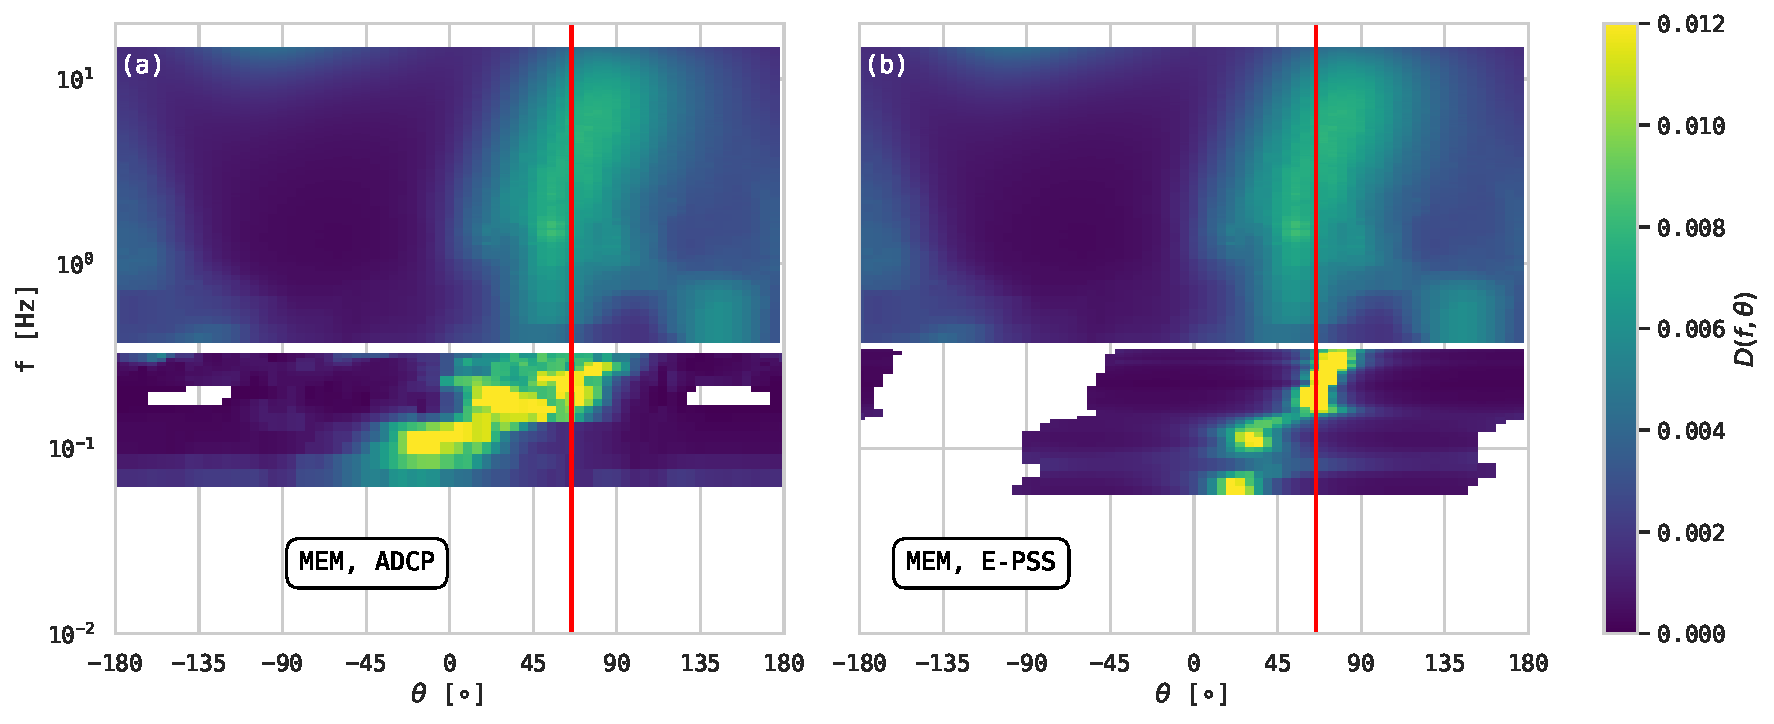
\includegraphics[width=\textwidth]{_figures/directional_spectra_combined.pdf}
    \vspace{-20pt}
\caption{Frequency-directional wave distribution $D(f,\theta)$ corresponding to the case shown in Figure \ref{fig:directional_spectra_polar}: (a) ADCP via MEM, (b) E-PSS via MEM, and (top half of a,b) directly from the wave slope field 3D Fourier transform. The red line indicates the wind direction in \lq\lq going-to" convention.}
\label{fig:directional_spectra_combined}
\end{figure*}

A pair of example frequency-directional wave spectra is shown in Figure \ref{fig:directional_spectra_polar}. The left panel contains the directional wave spectrum obtained from our Teledyne RDI Sentinel V ADCP \cite{herbers_field_1991}, while the right panel contains the directional wave spectrum inferred from the surface elevation and slope measurements of E-PSS. Each spectrum was produced using the maximum entropy method (MEM) \cite{lygre_maximum_1986}. Color corresponds to the base 10 logarithm of the spectral energy density. The black arrow gives the direction of the wind, while the red arrow provides the direction of the near surface current.

Given the frequency-directional spectrum $F(f,\theta)$,

\newpage

the wave directional distribution $D(f,\theta)$ is defined as:
\begin{align}
    D(f,\theta)\equiv \frac{F(f,\theta)}{F(f)}
\end{align}
% ... with $F(f)$ the omnidirectional frequency spectrum
... where $F(f)=\int_{-\pi}^{\pi}F(f,\theta)\mathrm{d}\theta$ is the omnidirectional frequency spectrum. Figure \ref{fig:directional_spectra_combined} contains $D(f,\theta)$ computed from the frequency-directional spectra shown in Figure \ref{fig:directional_spectra_polar}. The top portion of panels (a-b) correspond to the frequency directional spectra obtained directly from the water surface slope field \lq\lq stacks". The bottom portion of those panels correspond to the directional spectra obtained via MEM from either the ADCP or E-PSS measurement.

\newpage

Following Lin \emph{et al.} [2021] \cite{lin_estimating_2022}, we calculate mean wave direction $\theta_0$
\begin{align}
    \theta_0(f)=\int\limits_{-\pi}^{\pi}\theta D(f,\theta)\mathrm{d}\theta
    \label{eq:mean_wave_direction}
\end{align}
... and spreading width $\sigma_\theta$
\begin{align}
    \sigma_\theta(f)=\Bigg[\int\limits_{-\pi}^{\pi}\big(\theta-\theta_0\big)^2 D(f,\theta)\mathrm{d}\theta\Bigg]^{1/2}
\label{eq:spreading_width}
\end{align}

\vspace{-20pt}

\begin{figure}[!ht]
    \centering
    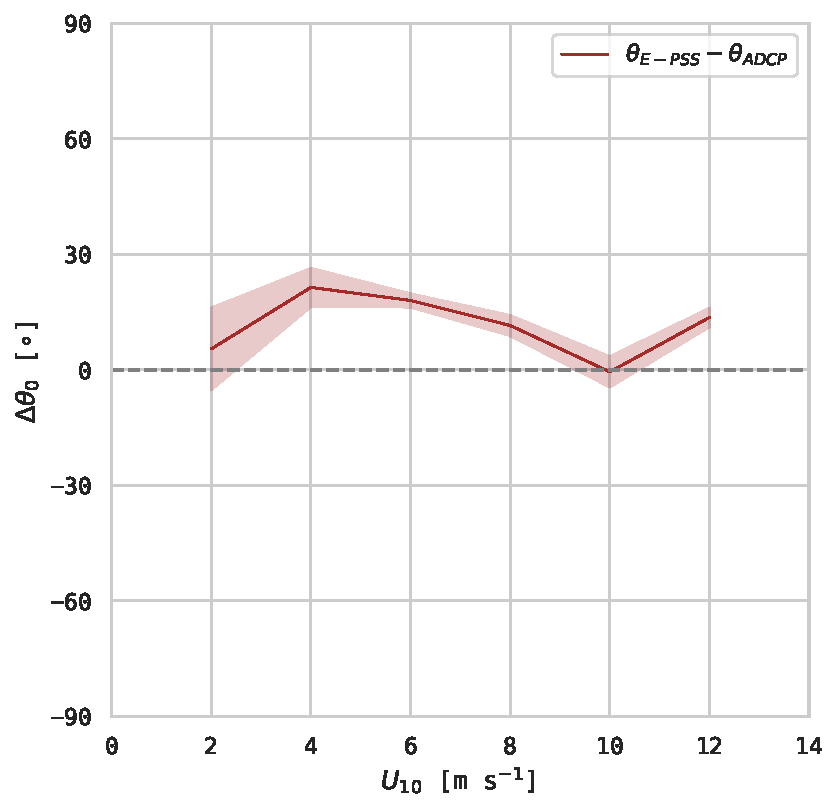
\includegraphics[width=0.49\textwidth]{_figures/delta_theta_nought.pdf}
    \caption{Difference in mean wave direction $\theta_0$ computed from ADCP and E-PSS directional spectra.}
    \label{fig:delta_theta_nought}
\end{figure}

\begin{figure*}[!hb]
    \centering
    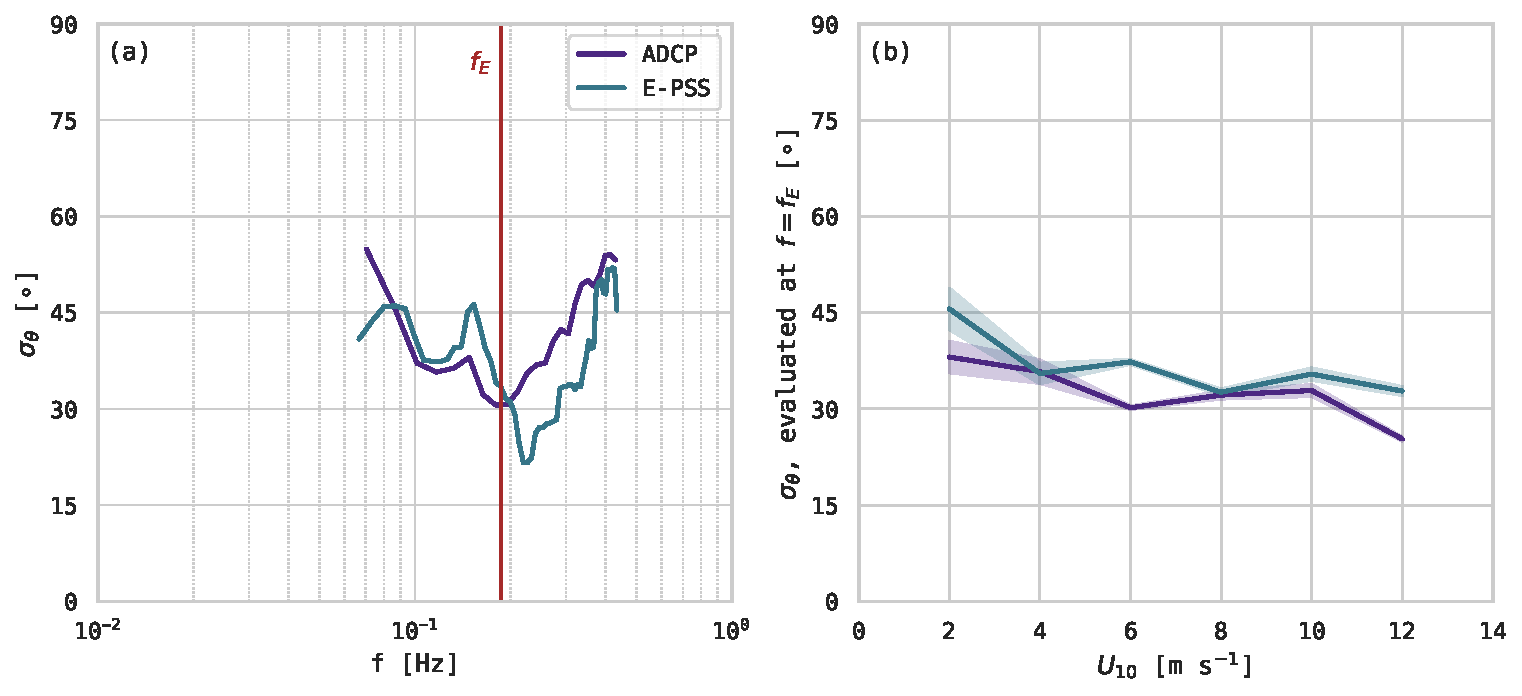
\includegraphics[width=\textwidth]{_figures/directional_spreading_comparison.pdf}
    \vspace{-20pt}
\caption{Spreading width $\sigma_\theta$, computed from $D(f,\theta)$ obtained from ADCP and E-PSS spectra following eq. \ref{eq:spreading_width} for (a) a single case (the one shown in Figures \ref{fig:directional_spectra_polar}-\ref{fig:directional_spectra_combined}) and given in terms of frequency and (b) all cases, bin-averaged and evaluated at the energy-weighted mean frequency $f_E$; shaded regions demarcate 95\% confidence intervals about the mean.}
\label{fig:directional_spreading_comparison}
\end{figure*}

The mean wave direction and directional spread may alternatively be computed from the first-order Fourier moments \cite{earle_nondirectional_2003}. However, we computed $\theta_0(f)$ and $\sigma_\theta(f)$ from the spectra themselves in order to maintain consistency of approach between the ADCP and E-PSS datasets. This approach carries the additional benefit that it would also be usable with the \lq\lq direct" frequency-directional spectra obtained from the wave slope fields themselves.

In Figure \ref{fig:delta_theta_nought}, we show the difference in mean wave direction $\Delta\theta_0$, with each $\theta_0$ computed from the ADCP and E-PSS directional spectra via equation \ref{eq:mean_wave_direction}. Values of $\Delta\theta$ were bin-averaged by ten-meter wind speed $U_{10}$, with bin centers/spacing following the convention used here up to this point. The red shaded region marks the 95\% confidence interval about the mean. Equation \ref{eq:spreading_width} provides the means to compute the wave directional spreading width $\sigma_\theta(f)$. A direct intercomparison of mean wave direction estimates does strain our capability: there is a substantial spatial separation ($\approx$1 km laterally) between the ADCP mooring and ASIT. More to the point, the ADCP mooring was on the 18.3-meter isobath while ASIT is on the 15-meter isobath. We attempted to correct for the latter effect (assuming simple refraction) via Snell's law, though this correction appears to have been negligible. In Figure \ref{fig:directional_spreading_comparison}(a), we show an example $\sigma_\theta(f)$ computed from the spreading functions $D(f,\theta)$ obtained by ADCP and E-PSS for a particular run. The red vertical segment corresponds to the frequency the energy-weighted mean frequency, $f_E=m_{-1}/m_{0}$. In panel (b), we provide the bin averaged response of $\sigma_\theta(f_E)$ as a function of 10 meter wind speed $U_{10}$. Shaded regions correspond to the 95\% confidence intervals about the mean.

\newpage

% ~\clearpage

\section{Discussion}
\label{sec:discussion}

\subsection{Core findings of this paper}

The results shown in Figure \ref{fig:Hm0_comparison_lidar_epss} ($H_{m0}$) and Figure \ref{fig:mss_upwind_crosswind} ($mss$) demonstrate that it is essential to characterize the polarization response of one's polarimetric camera-- and that failure to properly account for ambient environmental conditions may have a substantial negative impact on the measured slope magnitude. Our simple, single-camera \lq\lq empirical" correction to the observed DoLP allows E-PSS to provide a reasonable estimate of the significant wave height $H_{m0}$. A recent intercomparison \cite{jensen_quantifying_2021} between directional wave spectral estimates provided by different types of wave buoy systems (e.g., NOAA 3DMG, HIPPY, Triaxys, Watchman, and Datawell DWR) showed that for $H_{m0}$, it is reasonable to expect biases of approximately 0.1 m and RMSE of approximately 0.3 m. These values are almost exactly the error metrics we find for E-PSS relative to our reference lidar system, despite the enormous disparity in sample size between the two studies (order 10$^4$ for the buoy study, order 10$^2$ here). The buoy intercomparison estimates of mean wave period $T_{m02}$ are far more closely clustered than our E-PSS and lidar values, though we attribute the underestimation of mean wave period to the slight underestimation of wave energy at very low frequencies (as described in section \ref{sec:results}).

The empirical gain approach appears to improve the estimate of mean square slope (Figure \ref{fig:mss_upwind_crosswind}), though our observed values are still lower than classic observations \cite{Cox1954a,Breon2006} for moderate wind speeds ($U_{10}\geq7$ m s$^{-1}$). It may be the case that these relatively low values of $mss$ are owed to a degraded effective resolution of our polarimeter: for division of focal plane (DoFP) polarimeters like the one used in this study, one should expect a steep falloff in spectral energy density for scales 5-10 times larger than the image resolution \cite{laxague_effects_2025}. We have computed the upwind and crosswind slope variance from the model wavenumber-directional spectrum of Elfouhaily \emph{et al.} [1997] \cite{Elfouhaily1997}, setting the wavenumber upper limit of integration to 100 rad m$^{-1}$. It appears that this effective resolution limitation \cite{laxague_effects_2025} is a reasonable explanation for the relatively low wave slope variance observed here. The marginal wave slope PDFs (Figure \ref{fig:slope_distributions_binned_by_wind}) reveal that slopes with absolute value greater than 0.3 are extraordinarily rare at moderate wind forcing, even with the empirical DoLP gain. Waves of such extreme slopes tend to be exceptionally short-- e.g., sub-centimeter, in the short gravity-capillary and pure capillary regime. This low level of detection of ultra-steep waves is further evidence that the shortest waves are systematically underresolved \cite{laxague_effects_2025}. In contrast, the sun glint-based statistical results of Cox \& Munk and Br\'eon \& Henriot capture the total effect of surface waves to contribute to reflectance-- though those results do not provide insight into the scale dependence of the reflectance. It is this scale awareness of E-PSS---both in space and time---that makes the technique so valuable.

Higher-order statistics (skewness and kurtosis) were estimated from the coefficients inferred through a least-squares fit of a Gram-Charlier expansion to the 2D Gaussian wave slope distribution; these are provided in Figure \ref{fig:slope_distribution_GC_coeffs}. The effect of the DoLP gain on the computed wave slope skewness and kurtosis is inconclusive; it may be that the modest binned sample size of the present dataset (Figure \ref{fig:slope_distribution_GC_coeffs}) is insufficient to the task of parsing the behavior of these higher-order statistics given fine-grain adjustments to the measured light polarization state. Indeed, there is significant uncertainty in those parameters even as obtained from the large sample size satellite dataset used by Br\'eon \& Henriot [2006]. Nevertheless, the skewness and kurtosis values produced from the ASIT2019 field campaign are generally comparable to the classically-accepted values.

The combined omnidirectional spectra provided in Figure \ref{fig:omnidirectional_spectra_binned_by_wind} demonstrate the dual capabilities of E-PSS in providing a reliable measurement of both short waves and long waves. The polarization measurements used to compute the slope fields from which the spectra were produced were subjected to the empirically-derived DoLP gain. However, no further adjustments to the spectra were performed. The strong agreement in both spectral energy density and spectral subrange slope between the \lq\lq direct" omnidirectional spectra and those inferred from the long wave time series is a natural consequence of the internal consistency of E-PSS.

We sought to examine the ability of E-PSS to recover long wave directionality by computing the frequency-directional spectrum via MEM \cite{lygre_maximum_1986} given the two-component wave slope and water surface elevation. Use of an established technique like MEM confines our focus to the task of evaluating E-PSS itself. However, we note that the outputs of two-component wave slope and water surface elevation affords the technique a great deal of flexibility with respect to ultimate application. In particular, it opens E-PSS to a wide range of tools for evaluating wave directionality, including novel open-source utilities with the ability to capture nonstationarity in the wave field \cite{pelaez-zapata_ocean_2024,pelaez-zapata_ewdm_2025}

The wave frequency directional spectra shown in Figures \ref{fig:directional_spectra_polar} \& \ref{fig:directional_spectra_combined} provide a snapshot into the performance of E-PSS for capturing long wave directionality. Although it is difficult to say for certain without a third reference measurement, the smearing which occurs at the peak frequency in the ADCP-derived directional spectrum is likely a limitation of that particular measurement, whereas the directional veering we see in the E-PSS-derived spectra appears to track from the dominant long wave direction into the wind direction for shorter scales. As shown in Figure \ref{fig:directional_spectra_combined}, this alignment of intermediate-to-short gravity wave scales into the wind direction is consistent between the long wave and short wave (\lq\lq direct") portions of the E-PSS spectra. It is reasonable to expect some difference in mean wave direction between the ADCP-derived and E-PSS-derived spectra. In Figure \ref{fig:delta_theta_nought}, we see that this deviation is largest for low to moderate levels of wind forcing, but quite small (reliably less than 10$^{\circ}$ for higher levels of wind forcing ($U_{10}\geq$ 8 m s$^{-1}$). We note that the aforementioned buoy intercomparison \cite{jensen_quantifying_2021} found a mean difference in Fourier coefficient-derived $\bar{\theta}$ (analogous to our $\theta_0$) between buoys in the same location of $\approx$9$^{\circ}$. The directional spreading width at the energy-weighted mean frequency---i.e., $\sigma_\theta(f_E)$---determined via E-PSS is within 10$^{\circ}$ of the ADCP-derived estimate on average; furthermore, both estimates tend to follow the same general narrowing trend with wind speed ($\approx$1.5$^{\circ}$/(m s$^{-1}$)). Although the locations and periods of operation are entirely different, this range of wave directional spread is consistent with values typically observed at the USACE FRF 8-m array \cite{collins_performance_2024}, with $\sigma_\theta(f)$ ranging from 25$^{\circ}$ at 0.1-0.12 Hz to 45$^{\circ}$ at 0.25 Hz.

\subsection{Impact on existing literature}

The superior performance of the empirical DoLP correction (relative to no correction and a solely laboratory-based correction) is part blessing and part curse. On the one hand, it offers a way to ensure that existing datasets obtained with single surface-looking polarimeters may produce results which are robust to external environmental factors. However, it also indicates that previous applications of PSS---which did not take steps to account for variation in ambient illumination---may need to be reevaluated in light of the present results. Based on our review of existing literature on the topic (much of it contributed by the authors of this paper), we find a range of potential impacts. The studies most negatively impacted by a systematic underestimation of surface wave slope (and amplified case-to-case variability) are those with results based on the absolute spectral energy density or integrated slope variance at short gravity and gravity-capillary scales. These include field observations made with no laboratory calibration \cite{Laxague2015} and field observations made with a laboratory calibration \cite{Zappa2012,Laxague2018b}. However, in each of these cases, only a subset of the results were tied to the absolute magnitude of the slope spectral energy density. Many key results were based on the analysis of relative wave response, be it to hydrodynamic modulation \cite{Laxague2017a} or suppression by surfactant slicks \cite{laxague_suppression_2024}. Many of the applications of PSS have bypassed this issue entirely, using the spatiotemporal propagation of the waves simply as a means to obtain the near-surface current \cite{laxague2017b,Laxague2018a,Laxague2020a,Laxague2020b}; these results are entirely unaffected by the considerations mentioned here.

\subsection{Going forward}
\label{sec:forward}

In section \ref{sec:intro}, we stated that the most complete form of PSS would entail simultaneous measurement of the sky-leaving, upwelling, and surface-reflected polarization state. Crucially, this would require an in-water sensor for obtaining measurements of upwelling radiance. It may be feasible to obtain a functionally similar base of information from two cameras, both surface-looking: (1) one with a field of view (FOV) determined by the wave scales one desires to resolve and (2) one with a wide FOV, broad enough to capture angles of incidence ranging from near-nadir to past Brewster's angle ($\approx$53$^{\circ}$ for an air-water interface). The in-frame angles of incidence $\theta_i$ would be determined from the camera-lens combination's intrinsic and extrinsic parameters (i.e., through simple geometry). The wide-FOV polarimeter would then measure the variation of DoLP with $\theta_i$ that is particular to a given measurement; this would inherently include all effects related to the intensity and polarization state of sky-leaving and upwelling radiance. This field-determined DoLP($\theta_i$) would then be used as a 'lookup-table', allowing one to directly compute DoLP in the narrow-FOV scene without reliance on dedicated measurements or modeling of sky-leaving/upwelling radiance \cite{foster_characterization_2015,foster_polarized_2016} or any assumptions of theory. A demonstration of the sort of measurement which would enable this computation is provided in Figure \ref{fig:DoLP_AOI_field}. These observations were made on two non-consecutive days in Fall 2025 from the end of the pier in Piermont, NY, USA (incidentally, the same location used for the field validation exercise of Zappa \emph{et al.} [2008], \cite{Zappa2008}).

\begin{figure}[!ht]
    \centering
    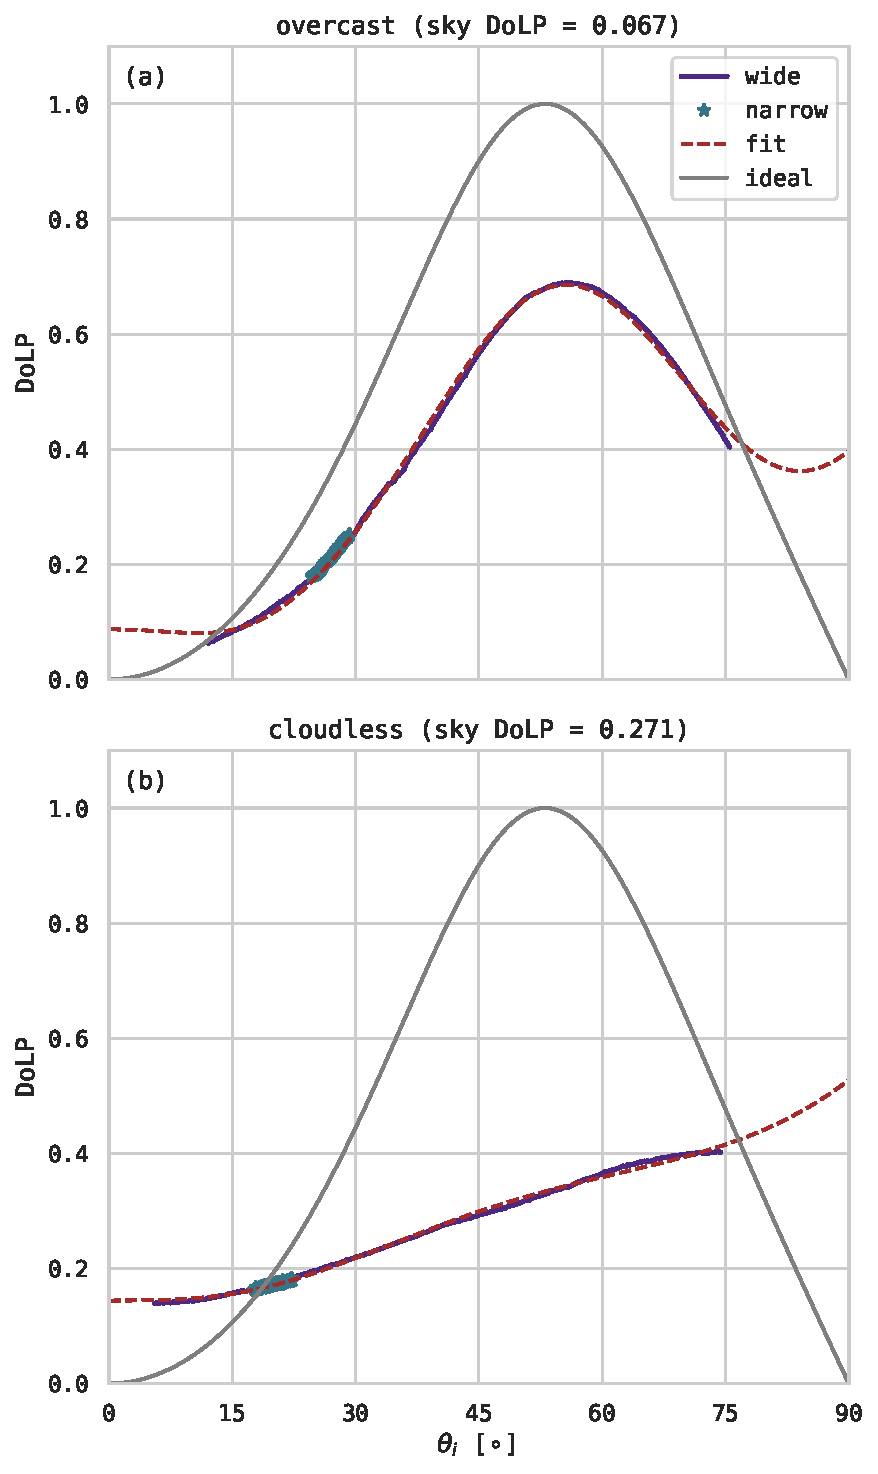
\includegraphics[width=0.49\textwidth]{_figures/DoLP_AOI_field.pdf}
    \vspace{-10pt}
    \caption{Variation of DoLP with $\theta_i$ observed on days with (a) overcast and (b) cloudless sky conditions. On the overcast day, the least-squares fit determined $\hat{S}_{sky}=[1.000,0.086,0.017]$ (DoLP = 0.087) with an upwelling fraction of 0.058. On the cloudless day, the least-squares fit determined $\hat{S}_{sky}=[1.000,0.117,0.084]$ (DoLP = 0.144) with an upwelling fraction of 0.140.}
    \label{fig:DoLP_AOI_field}
%    \vspace{-15pt}
\end{figure}

For this demonstration, we made use of two azimuthally-aligned polarimetric cameras with identical Sony Polarsens DoFP polarimetric detectors. One camera was fitted with a narrow FOV lens (75 mm focal length, angles of view 6.5$^{\circ}\times$5.4$^{\circ}$) and the other was fitted with a wide FOV lens (5 mm focal length, angles of view 80.7$^{\circ}\times$70.7$^{\circ}$). We found the mean DoLP measurements made by the two cameras to be comparable within their overlapping look region. Furthermore, in applying a least-squares fit to the data assuming a framework of specular reflection off the air-water interface, we were able to infer the Stokes vector of the sky-leaving radiance and the upwelling radiance fraction. It should be noted that the use of a wide-format lens may necessitate accounting for any effects resulting from light rays interacting obliquely with the polarizing filters on the focal plane array \cite{pistellato_geometric_2024}. In any case, further testing of this two-camera concept is left to a future study.

%\newpage

% ~\clearpage

\section{Summary}
\label{sec:summary}

We have presented an extension of the polarimetric slope sensing (PSS) technique for measuring ocean surface waves. This technique has been named \lq\lq extended polarimetric slope sensing", or E-PSS; the \lq\lq extended" modifier here denotes additional steps taken to 

\begin{enumerate}
    \item account for variation in ambient environmental conditions
    \item allow one to infer the directional characteristics of surface gravity waves many times larger than the polarimeter field of view
\end{enumerate}

\noindent When E-PSS is used with a simple empirical correction to the measured degree of linear polarization (DoLP), it is able to provide an accurate remote determination of the omnidirectional frequency spectrum across a wide range of surface wave frequencies (and therefore key sea state parameters, e.g. $H_{m0}$) from a single surface-looking imaging polarimeter. Further processing of the E-PSS outputs of water surface elevation and two-dimensional surface tilt yields a frequency-directional spectrum which is comparable to the spectrum obtained via a traditional ADCP-based approach. Crucially, these measurements are robust with respect to the ambient illumination condition. We find consistency in spectral energy density and equilibrium range slope between the long wave and short wave components of the omnidirectional frequency spectra produced by E-PSS. Furthermore, the short wave statistics obtained directly from the wave slope fields after empirical DoLP correction exhibit stronger agreement with classic observations than has been shown with the unadjusted results of previous applications of PSS. Finally, we present in concept an extension of this technique to involve two surface looking cameras, allowing for direct (in-scene) determination of the relationship between observed polarization state and surface inclination. This extension may improve performance in situations when the sky-leaving polarization state cannot be neglected, though that remains to be demonstrated at scale.

% use section* for acknowledgment
\section*{Acknowledgment}

The ASIT2019 field observations were made with the assistance of Steve Faluotico, Jay Sisson, the crew of the \textit{R/V Tioga}, and Carson Witte \& Suki Wong. We thank Alejandro Cifuentes-Lorenzen for sharing the ADCP directional wave spectra used here. Collection of field data from ASIT was supported by NSF (Award Number 1756839), ONR (Award Number N00014-22-1-2183), and NASA (Award Number 80NSSC19K1397). Analysis of the ASIT2019 dataset was supported by NSF award 20-49578 (NJML \& CJZ). NJML was also supported by NSF award 23-40712.

The full suite of codes which contain our implementation of Polarimetric Slope Sensing (PSS) for DoFP polarimeters (as well as the additional modules which comprise E-PSS) are available at \url{https://github.com/unh-cassll/polarimetric-slope-sensing}. All of the codes used to produce the graphics shown in this document are available within the following self-contained GitHub repository: \url{https://github.com/unh-cassll/E-PSS_paper}. These codes make use of data products stored at \textcolor{red}{DATA REPO (ZENODO)}.

\newpage

% references section

\bibliographystyle{IEEEtran}
\bibliography{references}

\begin{IEEEbiography}[{
\includegraphics[width=1in,height=1.25in,clip,keepaspectratio]{_figures/headshot_laxague.jpg}}]{Nathan J. M. Laxague}
(M '16) earned a Bachelor of Science in Physics in 2011 from the University of Miami, Coral Gables, FL USA. He received his Ph.D. in Applied Marine Physics from the Rosenstiel School of Marine and Atmospheric Sciences at the University of Miami in 2016. He was a postdoctoral research scientist at Lamont-Doherty Earth Observatory of Columbia University, in Palisades, NY, USA from 2017-2020. Since 2020, he has been an Assistant Professor of Ocean Engineering in the Department of Mechanical Engineering at the University of New Hampshire in Durham, NH, USA.
\end{IEEEbiography}

\begin{IEEEbiography}
[{
\includegraphics[width=1in,height=1.25in,clip,keepaspectratio]{_figures/headshot_duvarci.jpg}}]{Z. G\"oksu Duvarc\i}
earned a Bachelor of Science in Chemical Engineering with a Minor in Mechanical Engineering in 2022 from Bo\v gazi\c ci University in Istanbul, Turkey. She is currently a Ph.D. student in Ocean Engineering at the University of New Hampshire in Durham, NH, USA.
\end{IEEEbiography}

\begin{IEEEbiography}[{
\includegraphics[width=1in,height=1.25in,clip,keepaspectratio]{_figures/headshot_hogan.jpg}}]{Lindsay Hogan}
(M '24) earned a Bachelor of Science in Geology and Geophysics in 2020 from Yale University, New Haven, CT, USA. She received a Masters by Research in Climate and Atmospheric Science in 2021 from the University of Leeds, Leeds, UK. Lindsay earned a Master of Arts in Earth and Environmental Sciences from Columbia University in New York, NY, USA in 2023 and is currently a Ph.D. Candidate in Earth and Environmental Sciences at Columbia University and Lamont-Doherty Earth Observatory in Palisades, NY, USA.
\end{IEEEbiography}

\begin{IEEEbiography}[{
\includegraphics[width=1in,height=1.25in,clip,keepaspectratio]{_figures/headshot_liu.jpg}}]{Junzhe Liu}
(M '25) earned a Bachelor of Science in Oceanography in 2022 from University of Washington, Seattle, WA, USA. He earned a Master of Arts in Earth and Environmental Sciences from Columbia University in New York, NY, USA in 2024 and is currently a Ph.D. Candidate in Earth and Environmental Sciences at Columbia University and Lamont-Doherty Earth Observatory in Palisades, NY, USA.
\end{IEEEbiography}

\begin{IEEEbiography}[{
\includegraphics[width=1in,height=1.25in,clip,keepaspectratio]{_figures/headshot_bouillon.jpg}}]{Christopher Bouillon} earned a Bachelor of Engineering (B.Eng.) in Electrical Engineering in 2016 from Université de Sherbrooke. He received his Masters of Science in Physics from Université Laval, at the Centre for Optics, Photonics and Lasers (COPL). He obtained his Professional Engineering title (P. Eng.) from l'Ordre des Ingénieurs du Québec in 2025. He is currently a Ph.D. Candidate in Physical Oceanography at l'Institut des Sciences de la Mer (ISMER) of the Université du Québec à Rimouski, and a Lecturer in the Department of Mathematics, Computer Science and Engineering.
\end{IEEEbiography}

\begin{IEEEbiography}[{
\includegraphics[width=1in,height=1.25in,clip,keepaspectratio]{_figures/headshot_zappa.jpg}}]{Christopher J. Zappa}
(M '03) earned a Bachelor of Science in Mechanical Engineering in 1992 from Columbia University, NY, NY, USA.  He received his Masters in Engineering in 1994 and his Ph.D. in Applied Ocean Physics in 1999 from the University of Washington, Seattle, WA, USA, and completed his Postdoctoral Scholar Award at the Woods Hole Oceanographic Institution in 2003 in Woods Hole, MA, USA. He is currently a Lamont Research Professor in and the Associate Director of Ocean and Climate Physics at Lamont-Doherty Earth Observatory in Palisades, NY, USA, and a Lecturer in the Department of Earth and Environmental Sciences in NY, NY, USA, both at Columbia University.
\end{IEEEbiography}

\end{document}

